\documentclass[twoside]{book}

% Packages required by doxygen
\usepackage{fixltx2e}
\usepackage{calc}
\usepackage{doxygen}
\usepackage[export]{adjustbox} % also loads graphicx
\usepackage{graphicx}
\usepackage[utf8]{inputenc}
\usepackage{makeidx}
\usepackage{multicol}
\usepackage{multirow}
\PassOptionsToPackage{warn}{textcomp}
\usepackage{textcomp}
\usepackage[nointegrals]{wasysym}
\usepackage[table]{xcolor}

% Font selection
\usepackage[T1]{fontenc}
\usepackage[scaled=.90]{helvet}
\usepackage{courier}
\usepackage{amssymb}
\usepackage{sectsty}
\renewcommand{\familydefault}{\sfdefault}
\allsectionsfont{%
  \fontseries{bc}\selectfont%
  \color{darkgray}%
}
\renewcommand{\DoxyLabelFont}{%
  \fontseries{bc}\selectfont%
  \color{darkgray}%
}
\newcommand{\+}{\discretionary{\mbox{\scriptsize$\hookleftarrow$}}{}{}}

% Page & text layout
\usepackage{geometry}
\geometry{%
  a4paper,%
  top=2.5cm,%
  bottom=2.5cm,%
  left=2.5cm,%
  right=2.5cm%
}
\tolerance=750
\hfuzz=15pt
\hbadness=750
\setlength{\emergencystretch}{15pt}
\setlength{\parindent}{0cm}
\setlength{\parskip}{3ex plus 2ex minus 2ex}
\makeatletter
\renewcommand{\paragraph}{%
  \@startsection{paragraph}{4}{0ex}{-1.0ex}{1.0ex}{%
    \normalfont\normalsize\bfseries\SS@parafont%
  }%
}
\renewcommand{\subparagraph}{%
  \@startsection{subparagraph}{5}{0ex}{-1.0ex}{1.0ex}{%
    \normalfont\normalsize\bfseries\SS@subparafont%
  }%
}
\makeatother

% Headers & footers
\usepackage{fancyhdr}
\pagestyle{fancyplain}
\fancyhead[LE]{\fancyplain{}{\bfseries\thepage}}
\fancyhead[CE]{\fancyplain{}{}}
\fancyhead[RE]{\fancyplain{}{\bfseries\leftmark}}
\fancyhead[LO]{\fancyplain{}{\bfseries\rightmark}}
\fancyhead[CO]{\fancyplain{}{}}
\fancyhead[RO]{\fancyplain{}{\bfseries\thepage}}
\fancyfoot[LE]{\fancyplain{}{}}
\fancyfoot[CE]{\fancyplain{}{}}
\fancyfoot[RE]{\fancyplain{}{\bfseries\scriptsize Generated by Doxygen }}
\fancyfoot[LO]{\fancyplain{}{\bfseries\scriptsize Generated by Doxygen }}
\fancyfoot[CO]{\fancyplain{}{}}
\fancyfoot[RO]{\fancyplain{}{}}
\renewcommand{\footrulewidth}{0.4pt}
\renewcommand{\chaptermark}[1]{%
  \markboth{#1}{}%
}
\renewcommand{\sectionmark}[1]{%
  \markright{\thesection\ #1}%
}

% Indices & bibliography
\usepackage{natbib}
\usepackage[titles]{tocloft}
\setcounter{tocdepth}{3}
\setcounter{secnumdepth}{5}
\makeindex

% Hyperlinks (required, but should be loaded last)
\usepackage{ifpdf}
\ifpdf
  \usepackage[pdftex,pagebackref=true]{hyperref}
\else
  \usepackage[ps2pdf,pagebackref=true]{hyperref}
\fi
\hypersetup{%
  colorlinks=true,%
  linkcolor=blue,%
  citecolor=blue,%
  unicode%
}

% Custom commands
\newcommand{\clearemptydoublepage}{%
  \newpage{\pagestyle{empty}\cleardoublepage}%
}

\usepackage{caption}
\captionsetup{labelsep=space,justification=centering,font={bf},singlelinecheck=off,skip=4pt,position=top}

%===== C O N T E N T S =====

\begin{document}

% Titlepage & ToC
\hypersetup{pageanchor=false,
             bookmarksnumbered=true,
             pdfencoding=unicode
            }
\pagenumbering{alph}
\begin{titlepage}
\vspace*{7cm}
\begin{center}%
{\Large Gaze\+Track }\\
\vspace*{1cm}
{\large Generated by Doxygen 1.8.14}\\
\end{center}
\end{titlepage}
\clearemptydoublepage
\pagenumbering{roman}
\tableofcontents
\clearemptydoublepage
\pagenumbering{arabic}
\hypersetup{pageanchor=true}

%--- Begin generated contents ---
\chapter{Hierarchical Index}
\section{Class Hierarchy}
This inheritance list is sorted roughly, but not completely, alphabetically\+:\begin{DoxyCompactList}
\item Form\begin{DoxyCompactList}
\item \contentsline{section}{Gaze\+Track\+G\+UI\+:\+:Calibration\+Form}{\pageref{class_gaze_track_g_u_i_1_1_calibration_form}}{}
\item \contentsline{section}{Gaze\+Track\+G\+UI\+:\+:Feedback}{\pageref{class_gaze_track_g_u_i_1_1_feedback}}{}
\item \contentsline{section}{Gaze\+Track\+G\+UI\+:\+:G\+UI}{\pageref{class_gaze_track_g_u_i_1_1_g_u_i}}{}
\item \contentsline{section}{Gaze\+Track\+G\+UI\+:\+:Help\+Form}{\pageref{class_gaze_track_g_u_i_1_1_help_form}}{}
\item \contentsline{section}{Gaze\+Track\+G\+UI\+:\+:Tester}{\pageref{class_gaze_track_g_u_i_1_1_tester}}{}
\end{DoxyCompactList}
\item \contentsline{section}{Pupil\+Detect}{\pageref{class_pupil_detect}}{}
\item \contentsline{section}{Pupil\+Position}{\pageref{struct_pupil_position}}{}
\item \contentsline{section}{Tracker}{\pageref{class_tracker}}{}
\end{DoxyCompactList}

\chapter{Class Index}
\section{Class List}
Here are the classes, structs, unions and interfaces with brief descriptions\+:\begin{DoxyCompactList}
\item\contentsline{section}{\mbox{\hyperlink{class_gaze_track_g_u_i_1_1_calibration_form}{Gaze\+Track\+G\+U\+I\+::\+Calibration\+Form}} \\*Summary for \mbox{\hyperlink{class_gaze_track_g_u_i_1_1_calibration_form}{Calibration\+Form}} }{\pageref{class_gaze_track_g_u_i_1_1_calibration_form}}{}
\item\contentsline{section}{\mbox{\hyperlink{class_gaze_track_g_u_i_1_1_feedback}{Gaze\+Track\+G\+U\+I\+::\+Feedback}} \\*Summary for \mbox{\hyperlink{class_gaze_track_g_u_i_1_1_feedback}{Feedback}} }{\pageref{class_gaze_track_g_u_i_1_1_feedback}}{}
\item\contentsline{section}{\mbox{\hyperlink{class_gaze_track_g_u_i_1_1_g_u_i}{Gaze\+Track\+G\+U\+I\+::\+G\+UI}} }{\pageref{class_gaze_track_g_u_i_1_1_g_u_i}}{}
\item\contentsline{section}{\mbox{\hyperlink{class_gaze_track_g_u_i_1_1_help_form}{Gaze\+Track\+G\+U\+I\+::\+Help\+Form}} \\*Summary for \mbox{\hyperlink{class_gaze_track_g_u_i_1_1_help_form}{Help\+Form}} }{\pageref{class_gaze_track_g_u_i_1_1_help_form}}{}
\item\contentsline{section}{\mbox{\hyperlink{class_pupil_detect}{Pupil\+Detect}} }{\pageref{class_pupil_detect}}{}
\item\contentsline{section}{\mbox{\hyperlink{struct_pupil_position}{Pupil\+Position}} }{\pageref{struct_pupil_position}}{}
\item\contentsline{section}{\mbox{\hyperlink{class_gaze_track_g_u_i_1_1_tester}{Gaze\+Track\+G\+U\+I\+::\+Tester}} \\*Summary for \mbox{\hyperlink{class_gaze_track_g_u_i_1_1_tester}{Tester}} }{\pageref{class_gaze_track_g_u_i_1_1_tester}}{}
\item\contentsline{section}{\mbox{\hyperlink{class_tracker}{Tracker}} }{\pageref{class_tracker}}{}
\end{DoxyCompactList}

\chapter{Class Documentation}
\hypertarget{class_gaze_track_g_u_i_1_1_calibration_form}{}\section{Gaze\+Track\+G\+UI\+:\+:Calibration\+Form Class Reference}
\label{class_gaze_track_g_u_i_1_1_calibration_form}\index{Gaze\+Track\+G\+U\+I\+::\+Calibration\+Form@{Gaze\+Track\+G\+U\+I\+::\+Calibration\+Form}}


Summary for \mbox{\hyperlink{class_gaze_track_g_u_i_1_1_calibration_form}{Calibration\+Form}}  




{\ttfamily \#include $<$Calibration\+Form.\+h$>$}

Inheritance diagram for Gaze\+Track\+G\+UI\+:\+:Calibration\+Form\+:\begin{figure}[H]
\begin{center}
\leavevmode
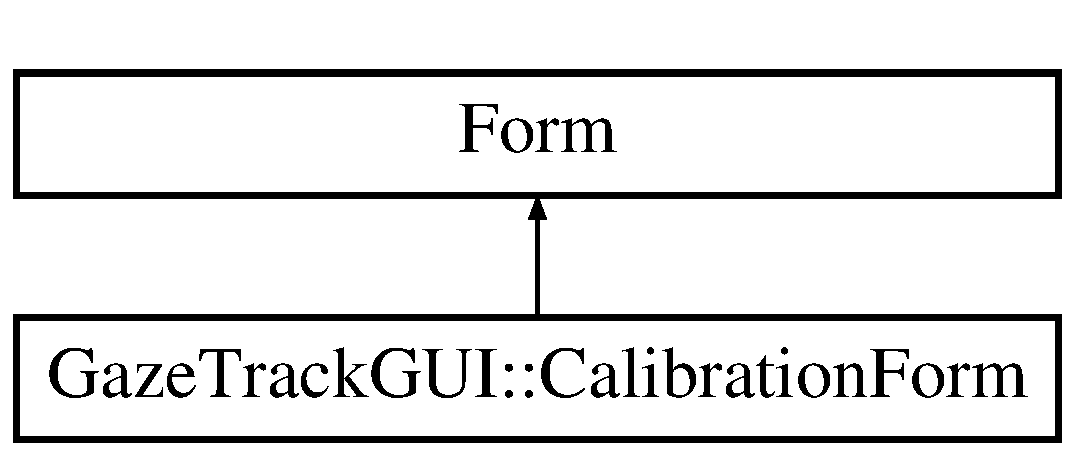
\includegraphics[height=2.000000cm]{class_gaze_track_g_u_i_1_1_calibration_form}
\end{center}
\end{figure}
\subsection*{Public Member Functions}
\begin{DoxyCompactItemize}
\item 
\mbox{\Hypertarget{class_gaze_track_g_u_i_1_1_calibration_form_ac09a90521622ec56819a249422a0e1d1}\label{class_gaze_track_g_u_i_1_1_calibration_form_ac09a90521622ec56819a249422a0e1d1}} 
void {\bfseries set\+Coordinates} ()
\end{DoxyCompactItemize}
\subsection*{Protected Member Functions}
\begin{DoxyCompactItemize}
\item 
\mbox{\hyperlink{class_gaze_track_g_u_i_1_1_calibration_form_a761b521b0ba7b8effae472f061f7fa2f}{$\sim$\+Calibration\+Form}} ()
\begin{DoxyCompactList}\small\item\em Clean up any resources being used. \end{DoxyCompactList}\end{DoxyCompactItemize}
\subsection*{Private Member Functions}
\begin{DoxyCompactItemize}
\item 
void \mbox{\hyperlink{class_gaze_track_g_u_i_1_1_calibration_form_a414b2f5880e33c407c2d598e7e1d8c23}{Initialize\+Component}} (void)
\begin{DoxyCompactList}\small\item\em Required method for Designer support -\/ do not modify the contents of this method with the code editor. \end{DoxyCompactList}\item 
\mbox{\Hypertarget{class_gaze_track_g_u_i_1_1_calibration_form_aa7c90a85f572b1f0adfcd6b217f3ce02}\label{class_gaze_track_g_u_i_1_1_calibration_form_aa7c90a85f572b1f0adfcd6b217f3ce02}} 
System\+::\+Void {\bfseries Calibration\+Form\+\_\+\+Load} (System\+::\+Object$^\wedge$ sender, System\+::\+Event\+Args$^\wedge$ e)
\item 
System\+::\+Void \mbox{\hyperlink{class_gaze_track_g_u_i_1_1_calibration_form_adea20c0c403187714e43d4e45dfa7e6a}{done\+Btn\+\_\+\+Click}} (System\+::\+Object$^\wedge$ sender, System\+::\+Event\+Args$^\wedge$ e)
\end{DoxyCompactItemize}
\subsection*{Private Attributes}
\begin{DoxyCompactItemize}
\item 
\mbox{\Hypertarget{class_gaze_track_g_u_i_1_1_calibration_form_acb52ab4255a9b1ebad2d7a7548fd124b}\label{class_gaze_track_g_u_i_1_1_calibration_form_acb52ab4255a9b1ebad2d7a7548fd124b}} 
System\+::\+Windows\+::\+Forms\+::\+Label $^\wedge$ {\bfseries label1}
\item 
\mbox{\Hypertarget{class_gaze_track_g_u_i_1_1_calibration_form_a931a052a51e02418d5115c749592ac97}\label{class_gaze_track_g_u_i_1_1_calibration_form_a931a052a51e02418d5115c749592ac97}} 
System\+::\+Windows\+::\+Forms\+::\+Label $^\wedge$ {\bfseries label2}
\item 
\mbox{\Hypertarget{class_gaze_track_g_u_i_1_1_calibration_form_a5a682a5e8eebd7614b8ff5128f44e08f}\label{class_gaze_track_g_u_i_1_1_calibration_form_a5a682a5e8eebd7614b8ff5128f44e08f}} 
System\+::\+Windows\+::\+Forms\+::\+Picture\+Box $^\wedge$ {\bfseries picture\+Box1}
\item 
\mbox{\Hypertarget{class_gaze_track_g_u_i_1_1_calibration_form_ac894ae8e225446ccdba65cc581fc0f10}\label{class_gaze_track_g_u_i_1_1_calibration_form_ac894ae8e225446ccdba65cc581fc0f10}} 
System\+::\+Windows\+::\+Forms\+::\+Picture\+Box $^\wedge$ {\bfseries picture\+Box2}
\item 
\mbox{\Hypertarget{class_gaze_track_g_u_i_1_1_calibration_form_a962a3043f1f929981cae3d4e46276049}\label{class_gaze_track_g_u_i_1_1_calibration_form_a962a3043f1f929981cae3d4e46276049}} 
System\+::\+Windows\+::\+Forms\+::\+Picture\+Box $^\wedge$ {\bfseries picture\+Box3}
\item 
\mbox{\Hypertarget{class_gaze_track_g_u_i_1_1_calibration_form_ad49d937d4e45ec7f9040a0599340cada}\label{class_gaze_track_g_u_i_1_1_calibration_form_ad49d937d4e45ec7f9040a0599340cada}} 
System\+::\+Windows\+::\+Forms\+::\+Picture\+Box $^\wedge$ {\bfseries picture\+Box4}
\item 
\mbox{\Hypertarget{class_gaze_track_g_u_i_1_1_calibration_form_a247f0056cbd3b7a8325233a0d8580d8a}\label{class_gaze_track_g_u_i_1_1_calibration_form_a247f0056cbd3b7a8325233a0d8580d8a}} 
System\+::\+Windows\+::\+Forms\+::\+Picture\+Box $^\wedge$ {\bfseries picture\+Box5}
\item 
\mbox{\Hypertarget{class_gaze_track_g_u_i_1_1_calibration_form_ae206d2412cc96644716cd5abd7276bf4}\label{class_gaze_track_g_u_i_1_1_calibration_form_ae206d2412cc96644716cd5abd7276bf4}} 
System\+::\+Windows\+::\+Forms\+::\+Picture\+Box $^\wedge$ {\bfseries picture\+Box6}
\item 
\mbox{\Hypertarget{class_gaze_track_g_u_i_1_1_calibration_form_a6fea8f937a8f72792e57a022032f0cbc}\label{class_gaze_track_g_u_i_1_1_calibration_form_a6fea8f937a8f72792e57a022032f0cbc}} 
System\+::\+Windows\+::\+Forms\+::\+Picture\+Box $^\wedge$ {\bfseries picture\+Box7}
\item 
\mbox{\Hypertarget{class_gaze_track_g_u_i_1_1_calibration_form_ab62a7952a180faa1a2a4ddb0e402bcbe}\label{class_gaze_track_g_u_i_1_1_calibration_form_ab62a7952a180faa1a2a4ddb0e402bcbe}} 
System\+::\+Windows\+::\+Forms\+::\+Picture\+Box $^\wedge$ {\bfseries picture\+Box8}
\item 
\mbox{\Hypertarget{class_gaze_track_g_u_i_1_1_calibration_form_a60e86d7bc5754ecca99e99be6a5941ab}\label{class_gaze_track_g_u_i_1_1_calibration_form_a60e86d7bc5754ecca99e99be6a5941ab}} 
System\+::\+Windows\+::\+Forms\+::\+Picture\+Box $^\wedge$ {\bfseries picture\+Box9}
\item 
\mbox{\Hypertarget{class_gaze_track_g_u_i_1_1_calibration_form_abcdfc02f5a5eb07862b07ead5a3f70b0}\label{class_gaze_track_g_u_i_1_1_calibration_form_abcdfc02f5a5eb07862b07ead5a3f70b0}} 
System\+::\+Windows\+::\+Forms\+::\+Label $^\wedge$ {\bfseries label4}
\item 
\mbox{\Hypertarget{class_gaze_track_g_u_i_1_1_calibration_form_a29aac4803970bfd922c356e5142b88d0}\label{class_gaze_track_g_u_i_1_1_calibration_form_a29aac4803970bfd922c356e5142b88d0}} 
System\+::\+Windows\+::\+Forms\+::\+Label $^\wedge$ {\bfseries label3}
\item 
\mbox{\Hypertarget{class_gaze_track_g_u_i_1_1_calibration_form_a62b03ce5a8059d9569ec46541a89cfc1}\label{class_gaze_track_g_u_i_1_1_calibration_form_a62b03ce5a8059d9569ec46541a89cfc1}} 
System\+::\+Windows\+::\+Forms\+::\+Label $^\wedge$ {\bfseries label5}
\item 
\mbox{\Hypertarget{class_gaze_track_g_u_i_1_1_calibration_form_ac5fb4f9c33e8750caeab9c29d2cb6b36}\label{class_gaze_track_g_u_i_1_1_calibration_form_ac5fb4f9c33e8750caeab9c29d2cb6b36}} 
System\+::\+Windows\+::\+Forms\+::\+Label $^\wedge$ {\bfseries label6}
\item 
\mbox{\Hypertarget{class_gaze_track_g_u_i_1_1_calibration_form_a61fb87896cde1e3b5b346cf2cdd3fa5c}\label{class_gaze_track_g_u_i_1_1_calibration_form_a61fb87896cde1e3b5b346cf2cdd3fa5c}} 
System\+::\+Windows\+::\+Forms\+::\+Label $^\wedge$ {\bfseries label7}
\item 
\mbox{\Hypertarget{class_gaze_track_g_u_i_1_1_calibration_form_a067364d2f7669cd6e9125e908b048623}\label{class_gaze_track_g_u_i_1_1_calibration_form_a067364d2f7669cd6e9125e908b048623}} 
System\+::\+Windows\+::\+Forms\+::\+Label $^\wedge$ {\bfseries label8}
\item 
\mbox{\Hypertarget{class_gaze_track_g_u_i_1_1_calibration_form_a67bb80d457e1a8eb0d34061221f489dc}\label{class_gaze_track_g_u_i_1_1_calibration_form_a67bb80d457e1a8eb0d34061221f489dc}} 
System\+::\+Windows\+::\+Forms\+::\+Label $^\wedge$ {\bfseries label9}
\item 
\mbox{\Hypertarget{class_gaze_track_g_u_i_1_1_calibration_form_a537c831514ab4aa8b1c8ca28e4b2781f}\label{class_gaze_track_g_u_i_1_1_calibration_form_a537c831514ab4aa8b1c8ca28e4b2781f}} 
System\+::\+Windows\+::\+Forms\+::\+Label $^\wedge$ {\bfseries label10}
\item 
\mbox{\Hypertarget{class_gaze_track_g_u_i_1_1_calibration_form_a3e0a6ab03cc68c4f5a9c34ae29df4c97}\label{class_gaze_track_g_u_i_1_1_calibration_form_a3e0a6ab03cc68c4f5a9c34ae29df4c97}} 
System\+::\+Windows\+::\+Forms\+::\+Label $^\wedge$ {\bfseries label11}
\item 
\mbox{\Hypertarget{class_gaze_track_g_u_i_1_1_calibration_form_a55f84b550b25b650893ac7480f51eb90}\label{class_gaze_track_g_u_i_1_1_calibration_form_a55f84b550b25b650893ac7480f51eb90}} 
System\+::\+Windows\+::\+Forms\+::\+Button $^\wedge$ {\bfseries done\+Btn}
\item 
\mbox{\Hypertarget{class_gaze_track_g_u_i_1_1_calibration_form_a4af4ca8ba916ac8d207365031768a819}\label{class_gaze_track_g_u_i_1_1_calibration_form_a4af4ca8ba916ac8d207365031768a819}} 
System\+::\+Windows\+::\+Forms\+::\+Text\+Box $^\wedge$ {\bfseries name\+Box}
\item 
System\+::\+Component\+Model\+::\+Container $^\wedge$ \mbox{\hyperlink{class_gaze_track_g_u_i_1_1_calibration_form_a27cbe7b426a34ce1e7509ecf62a3d3a3}{components}}
\begin{DoxyCompactList}\small\item\em Required designer variable. \end{DoxyCompactList}\end{DoxyCompactItemize}


\subsection{Detailed Description}
Summary for \mbox{\hyperlink{class_gaze_track_g_u_i_1_1_calibration_form}{Calibration\+Form}} 



\subsection{Constructor \& Destructor Documentation}
\mbox{\Hypertarget{class_gaze_track_g_u_i_1_1_calibration_form_a761b521b0ba7b8effae472f061f7fa2f}\label{class_gaze_track_g_u_i_1_1_calibration_form_a761b521b0ba7b8effae472f061f7fa2f}} 
\index{Gaze\+Track\+G\+U\+I\+::\+Calibration\+Form@{Gaze\+Track\+G\+U\+I\+::\+Calibration\+Form}!````~Calibration\+Form@{$\sim$\+Calibration\+Form}}
\index{````~Calibration\+Form@{$\sim$\+Calibration\+Form}!Gaze\+Track\+G\+U\+I\+::\+Calibration\+Form@{Gaze\+Track\+G\+U\+I\+::\+Calibration\+Form}}
\subsubsection{\texorpdfstring{$\sim$\+Calibration\+Form()}{~CalibrationForm()}}
{\footnotesize\ttfamily Gaze\+Track\+G\+U\+I\+::\+Calibration\+Form\+::$\sim$\+Calibration\+Form (\begin{DoxyParamCaption}{ }\end{DoxyParamCaption})\hspace{0.3cm}{\ttfamily [inline]}, {\ttfamily [protected]}}



Clean up any resources being used. 



\subsection{Member Function Documentation}
\mbox{\Hypertarget{class_gaze_track_g_u_i_1_1_calibration_form_adea20c0c403187714e43d4e45dfa7e6a}\label{class_gaze_track_g_u_i_1_1_calibration_form_adea20c0c403187714e43d4e45dfa7e6a}} 
\index{Gaze\+Track\+G\+U\+I\+::\+Calibration\+Form@{Gaze\+Track\+G\+U\+I\+::\+Calibration\+Form}!done\+Btn\+\_\+\+Click@{done\+Btn\+\_\+\+Click}}
\index{done\+Btn\+\_\+\+Click@{done\+Btn\+\_\+\+Click}!Gaze\+Track\+G\+U\+I\+::\+Calibration\+Form@{Gaze\+Track\+G\+U\+I\+::\+Calibration\+Form}}
\subsubsection{\texorpdfstring{done\+Btn\+\_\+\+Click()}{doneBtn\_Click()}}
{\footnotesize\ttfamily System\+::\+Void Gaze\+Track\+G\+U\+I\+::\+Calibration\+Form\+::done\+Btn\+\_\+\+Click (\begin{DoxyParamCaption}\item[{System\+::\+Object$^\wedge$}]{sender,  }\item[{System\+::\+Event\+Args$^\wedge$}]{e }\end{DoxyParamCaption})\hspace{0.3cm}{\ttfamily [inline]}, {\ttfamily [private]}}

Gets the text that is entered in the name\+Box and saves it in the data.\+txt file \mbox{\Hypertarget{class_gaze_track_g_u_i_1_1_calibration_form_a414b2f5880e33c407c2d598e7e1d8c23}\label{class_gaze_track_g_u_i_1_1_calibration_form_a414b2f5880e33c407c2d598e7e1d8c23}} 
\index{Gaze\+Track\+G\+U\+I\+::\+Calibration\+Form@{Gaze\+Track\+G\+U\+I\+::\+Calibration\+Form}!Initialize\+Component@{Initialize\+Component}}
\index{Initialize\+Component@{Initialize\+Component}!Gaze\+Track\+G\+U\+I\+::\+Calibration\+Form@{Gaze\+Track\+G\+U\+I\+::\+Calibration\+Form}}
\subsubsection{\texorpdfstring{Initialize\+Component()}{InitializeComponent()}}
{\footnotesize\ttfamily void Gaze\+Track\+G\+U\+I\+::\+Calibration\+Form\+::\+Initialize\+Component (\begin{DoxyParamCaption}\item[{void}]{ }\end{DoxyParamCaption})\hspace{0.3cm}{\ttfamily [inline]}, {\ttfamily [private]}}



Required method for Designer support -\/ do not modify the contents of this method with the code editor. 



\subsection{Member Data Documentation}
\mbox{\Hypertarget{class_gaze_track_g_u_i_1_1_calibration_form_a27cbe7b426a34ce1e7509ecf62a3d3a3}\label{class_gaze_track_g_u_i_1_1_calibration_form_a27cbe7b426a34ce1e7509ecf62a3d3a3}} 
\index{Gaze\+Track\+G\+U\+I\+::\+Calibration\+Form@{Gaze\+Track\+G\+U\+I\+::\+Calibration\+Form}!components@{components}}
\index{components@{components}!Gaze\+Track\+G\+U\+I\+::\+Calibration\+Form@{Gaze\+Track\+G\+U\+I\+::\+Calibration\+Form}}
\subsubsection{\texorpdfstring{components}{components}}
{\footnotesize\ttfamily System\+::\+Component\+Model\+::\+Container $^\wedge$ Gaze\+Track\+G\+U\+I\+::\+Calibration\+Form\+::components\hspace{0.3cm}{\ttfamily [private]}}



Required designer variable. 



The documentation for this class was generated from the following files\+:\begin{DoxyCompactItemize}
\item 
F\+:/\+Gaze\+Track\+G\+U\+I/Calibration\+Form.\+h\item 
F\+:/\+Gaze\+Track\+G\+U\+I/Calibration\+Form.\+cpp\end{DoxyCompactItemize}

\hypertarget{class_gaze_track_g_u_i_1_1_feedback}{}\section{Gaze\+Track\+G\+UI\+:\+:Feedback Class Reference}
\label{class_gaze_track_g_u_i_1_1_feedback}\index{Gaze\+Track\+G\+U\+I\+::\+Feedback@{Gaze\+Track\+G\+U\+I\+::\+Feedback}}


Summary for \mbox{\hyperlink{class_gaze_track_g_u_i_1_1_feedback}{Feedback}}  




{\ttfamily \#include $<$Feedback.\+h$>$}

Inheritance diagram for Gaze\+Track\+G\+UI\+:\+:Feedback\+:\begin{figure}[H]
\begin{center}
\leavevmode
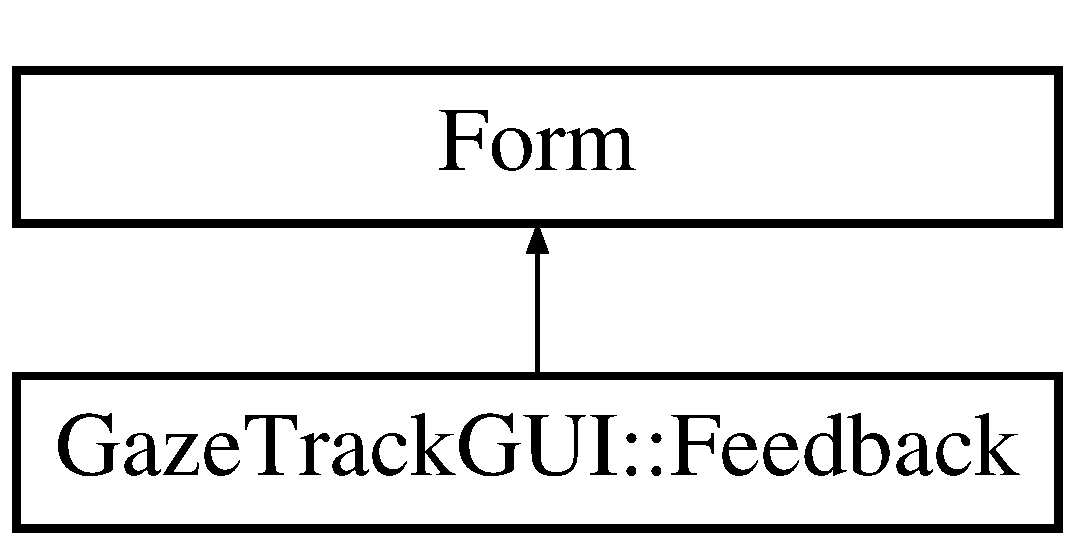
\includegraphics[height=2.000000cm]{class_gaze_track_g_u_i_1_1_feedback}
\end{center}
\end{figure}
\subsection*{Protected Member Functions}
\begin{DoxyCompactItemize}
\item 
\mbox{\hyperlink{class_gaze_track_g_u_i_1_1_feedback_ae57806d85cda496358ac7c2dc3b2b593}{$\sim$\+Feedback}} ()
\begin{DoxyCompactList}\small\item\em Clean up any resources being used. \end{DoxyCompactList}\end{DoxyCompactItemize}
\subsection*{Private Member Functions}
\begin{DoxyCompactItemize}
\item 
void \mbox{\hyperlink{class_gaze_track_g_u_i_1_1_feedback_a31c61a04fb35ae92344f9fa7e609aef4}{Initialize\+Component}} (void)
\begin{DoxyCompactList}\small\item\em Required method for Designer support -\/ do not modify the contents of this method with the code editor. \end{DoxyCompactList}\item 
\mbox{\Hypertarget{class_gaze_track_g_u_i_1_1_feedback_ac3924a149f409502ff26393084bf7c59}\label{class_gaze_track_g_u_i_1_1_feedback_ac3924a149f409502ff26393084bf7c59}} 
System\+::\+Void {\bfseries exit\+Btn\+\_\+\+Click} (System\+::\+Object$^\wedge$ sender, System\+::\+Event\+Args$^\wedge$ e)
\item 
\mbox{\Hypertarget{class_gaze_track_g_u_i_1_1_feedback_a1ec056911bbf5543910b61ea024f0b92}\label{class_gaze_track_g_u_i_1_1_feedback_a1ec056911bbf5543910b61ea024f0b92}} 
System\+::\+Void {\bfseries submit\+Btn\+\_\+\+Click} (System\+::\+Object$^\wedge$ sender, System\+::\+Event\+Args$^\wedge$ e)
\item 
\mbox{\Hypertarget{class_gaze_track_g_u_i_1_1_feedback_a3d6590b575892e4f512ad4ad172a63c6}\label{class_gaze_track_g_u_i_1_1_feedback_a3d6590b575892e4f512ad4ad172a63c6}} 
System\+::\+Void {\bfseries q1\+List\+\_\+\+Selected\+Index\+Changed} (System\+::\+Object$^\wedge$ sender, System\+::\+Event\+Args$^\wedge$ e)
\end{DoxyCompactItemize}
\subsection*{Private Attributes}
\begin{DoxyCompactItemize}
\item 
\mbox{\Hypertarget{class_gaze_track_g_u_i_1_1_feedback_adf7b95399622b5e4577430e518b22d87}\label{class_gaze_track_g_u_i_1_1_feedback_adf7b95399622b5e4577430e518b22d87}} 
System\+::\+Windows\+::\+Forms\+::\+Label $^\wedge$ {\bfseries label1}
\item 
\mbox{\Hypertarget{class_gaze_track_g_u_i_1_1_feedback_aafab7eebaf1702df586b4988ab779318}\label{class_gaze_track_g_u_i_1_1_feedback_aafab7eebaf1702df586b4988ab779318}} 
System\+::\+Windows\+::\+Forms\+::\+Button $^\wedge$ {\bfseries exit\+Btn}
\item 
\mbox{\Hypertarget{class_gaze_track_g_u_i_1_1_feedback_ae2dafe117d9b3c00c8006c9e6682d7cf}\label{class_gaze_track_g_u_i_1_1_feedback_ae2dafe117d9b3c00c8006c9e6682d7cf}} 
System\+::\+Windows\+::\+Forms\+::\+Button $^\wedge$ {\bfseries submit\+Btn}
\item 
\mbox{\Hypertarget{class_gaze_track_g_u_i_1_1_feedback_af949e1b5319f2526d7e02e79e3315d59}\label{class_gaze_track_g_u_i_1_1_feedback_af949e1b5319f2526d7e02e79e3315d59}} 
System\+::\+Windows\+::\+Forms\+::\+Label $^\wedge$ {\bfseries q1\+Lbl}
\item 
\mbox{\Hypertarget{class_gaze_track_g_u_i_1_1_feedback_ad7f462065808ff12c29df3010bab0ba1}\label{class_gaze_track_g_u_i_1_1_feedback_ad7f462065808ff12c29df3010bab0ba1}} 
System\+::\+Windows\+::\+Forms\+::\+Combo\+Box $^\wedge$ {\bfseries q1\+List}
\item 
\mbox{\Hypertarget{class_gaze_track_g_u_i_1_1_feedback_a6730740bc9b30bde05d03d0ed891abeb}\label{class_gaze_track_g_u_i_1_1_feedback_a6730740bc9b30bde05d03d0ed891abeb}} 
System\+::\+Windows\+::\+Forms\+::\+Combo\+Box $^\wedge$ {\bfseries q2\+List}
\item 
\mbox{\Hypertarget{class_gaze_track_g_u_i_1_1_feedback_af48b9f86110cf82505fe927fcbe409b0}\label{class_gaze_track_g_u_i_1_1_feedback_af48b9f86110cf82505fe927fcbe409b0}} 
System\+::\+Windows\+::\+Forms\+::\+Label $^\wedge$ {\bfseries q2\+Lbl}
\item 
\mbox{\Hypertarget{class_gaze_track_g_u_i_1_1_feedback_a99c9d629ca63fdae554e280100b65826}\label{class_gaze_track_g_u_i_1_1_feedback_a99c9d629ca63fdae554e280100b65826}} 
System\+::\+Windows\+::\+Forms\+::\+Label $^\wedge$ {\bfseries label4}
\item 
\mbox{\Hypertarget{class_gaze_track_g_u_i_1_1_feedback_a59f211443a85e0a10345fe3fc4685880}\label{class_gaze_track_g_u_i_1_1_feedback_a59f211443a85e0a10345fe3fc4685880}} 
System\+::\+Windows\+::\+Forms\+::\+Combo\+Box $^\wedge$ {\bfseries q3\+List}
\item 
\mbox{\Hypertarget{class_gaze_track_g_u_i_1_1_feedback_a319367eb4b5261efe2c621e4b1fff2f3}\label{class_gaze_track_g_u_i_1_1_feedback_a319367eb4b5261efe2c621e4b1fff2f3}} 
System\+::\+Windows\+::\+Forms\+::\+Label $^\wedge$ {\bfseries q3\+Lbl}
\item 
\mbox{\Hypertarget{class_gaze_track_g_u_i_1_1_feedback_a46bce8a7a95f4f1169662c889e36098f}\label{class_gaze_track_g_u_i_1_1_feedback_a46bce8a7a95f4f1169662c889e36098f}} 
System\+::\+Windows\+::\+Forms\+::\+Label $^\wedge$ {\bfseries label2}
\item 
\mbox{\Hypertarget{class_gaze_track_g_u_i_1_1_feedback_a31c12024aa7ddda4182aed5fce031e06}\label{class_gaze_track_g_u_i_1_1_feedback_a31c12024aa7ddda4182aed5fce031e06}} 
System\+::\+Windows\+::\+Forms\+::\+Combo\+Box $^\wedge$ {\bfseries q4\+List}
\item 
\mbox{\Hypertarget{class_gaze_track_g_u_i_1_1_feedback_a02a8f63e8968888c3c805d41500f205b}\label{class_gaze_track_g_u_i_1_1_feedback_a02a8f63e8968888c3c805d41500f205b}} 
System\+::\+Windows\+::\+Forms\+::\+Label $^\wedge$ {\bfseries q4\+Lbl}
\item 
\mbox{\Hypertarget{class_gaze_track_g_u_i_1_1_feedback_a21577db6aa9dbef15a90c8ef3c1c87b7}\label{class_gaze_track_g_u_i_1_1_feedback_a21577db6aa9dbef15a90c8ef3c1c87b7}} 
System\+::\+Windows\+::\+Forms\+::\+Combo\+Box $^\wedge$ {\bfseries q5\+List}
\item 
\mbox{\Hypertarget{class_gaze_track_g_u_i_1_1_feedback_a5199443ff35a81547d9fe949fff387d6}\label{class_gaze_track_g_u_i_1_1_feedback_a5199443ff35a81547d9fe949fff387d6}} 
System\+::\+Windows\+::\+Forms\+::\+Label $^\wedge$ {\bfseries q5\+Lbl}
\item 
System\+::\+Component\+Model\+::\+Container $^\wedge$ \mbox{\hyperlink{class_gaze_track_g_u_i_1_1_feedback_a26e51fa73149737460c9a20e9be9dfe2}{components}}
\begin{DoxyCompactList}\small\item\em Required designer variable. \end{DoxyCompactList}\end{DoxyCompactItemize}


\subsection{Detailed Description}
Summary for \mbox{\hyperlink{class_gaze_track_g_u_i_1_1_feedback}{Feedback}} 



\subsection{Constructor \& Destructor Documentation}
\mbox{\Hypertarget{class_gaze_track_g_u_i_1_1_feedback_ae57806d85cda496358ac7c2dc3b2b593}\label{class_gaze_track_g_u_i_1_1_feedback_ae57806d85cda496358ac7c2dc3b2b593}} 
\index{Gaze\+Track\+G\+U\+I\+::\+Feedback@{Gaze\+Track\+G\+U\+I\+::\+Feedback}!````~Feedback@{$\sim$\+Feedback}}
\index{````~Feedback@{$\sim$\+Feedback}!Gaze\+Track\+G\+U\+I\+::\+Feedback@{Gaze\+Track\+G\+U\+I\+::\+Feedback}}
\subsubsection{\texorpdfstring{$\sim$\+Feedback()}{~Feedback()}}
{\footnotesize\ttfamily Gaze\+Track\+G\+U\+I\+::\+Feedback\+::$\sim$\+Feedback (\begin{DoxyParamCaption}{ }\end{DoxyParamCaption})\hspace{0.3cm}{\ttfamily [inline]}, {\ttfamily [protected]}}



Clean up any resources being used. 



\subsection{Member Function Documentation}
\mbox{\Hypertarget{class_gaze_track_g_u_i_1_1_feedback_a31c61a04fb35ae92344f9fa7e609aef4}\label{class_gaze_track_g_u_i_1_1_feedback_a31c61a04fb35ae92344f9fa7e609aef4}} 
\index{Gaze\+Track\+G\+U\+I\+::\+Feedback@{Gaze\+Track\+G\+U\+I\+::\+Feedback}!Initialize\+Component@{Initialize\+Component}}
\index{Initialize\+Component@{Initialize\+Component}!Gaze\+Track\+G\+U\+I\+::\+Feedback@{Gaze\+Track\+G\+U\+I\+::\+Feedback}}
\subsubsection{\texorpdfstring{Initialize\+Component()}{InitializeComponent()}}
{\footnotesize\ttfamily void Gaze\+Track\+G\+U\+I\+::\+Feedback\+::\+Initialize\+Component (\begin{DoxyParamCaption}\item[{void}]{ }\end{DoxyParamCaption})\hspace{0.3cm}{\ttfamily [inline]}, {\ttfamily [private]}}



Required method for Designer support -\/ do not modify the contents of this method with the code editor. 



\subsection{Member Data Documentation}
\mbox{\Hypertarget{class_gaze_track_g_u_i_1_1_feedback_a26e51fa73149737460c9a20e9be9dfe2}\label{class_gaze_track_g_u_i_1_1_feedback_a26e51fa73149737460c9a20e9be9dfe2}} 
\index{Gaze\+Track\+G\+U\+I\+::\+Feedback@{Gaze\+Track\+G\+U\+I\+::\+Feedback}!components@{components}}
\index{components@{components}!Gaze\+Track\+G\+U\+I\+::\+Feedback@{Gaze\+Track\+G\+U\+I\+::\+Feedback}}
\subsubsection{\texorpdfstring{components}{components}}
{\footnotesize\ttfamily System\+::\+Component\+Model\+::\+Container $^\wedge$ Gaze\+Track\+G\+U\+I\+::\+Feedback\+::components\hspace{0.3cm}{\ttfamily [private]}}



Required designer variable. 



The documentation for this class was generated from the following file\+:\begin{DoxyCompactItemize}
\item 
F\+:/\+Gaze\+Track\+G\+U\+I/Feedback.\+h\end{DoxyCompactItemize}

\hypertarget{class_gaze_track_g_u_i_1_1_g_u_i}{}\section{Gaze\+Track\+G\+UI\+:\+:G\+UI Class Reference}
\label{class_gaze_track_g_u_i_1_1_g_u_i}\index{Gaze\+Track\+G\+U\+I\+::\+G\+UI@{Gaze\+Track\+G\+U\+I\+::\+G\+UI}}
Inheritance diagram for Gaze\+Track\+G\+UI\+:\+:G\+UI\+:\begin{figure}[H]
\begin{center}
\leavevmode
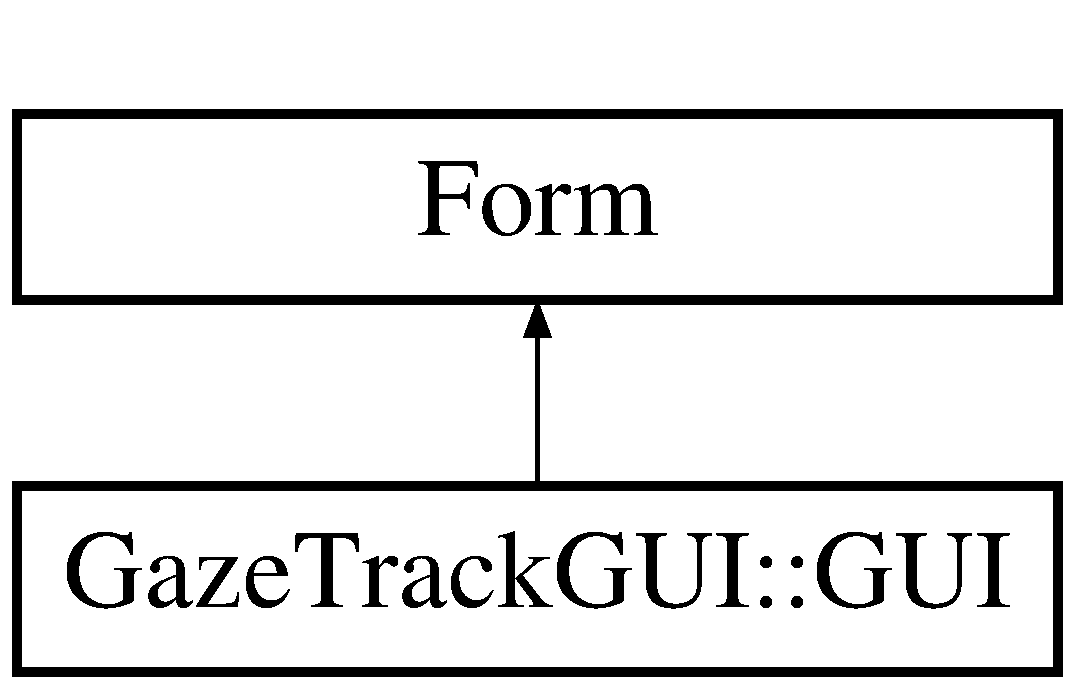
\includegraphics[height=2.000000cm]{class_gaze_track_g_u_i_1_1_g_u_i}
\end{center}
\end{figure}
\subsection*{Public Member Functions}
\begin{DoxyCompactItemize}
\item 
void \mbox{\hyperlink{class_gaze_track_g_u_i_1_1_g_u_i_a81f7231e79205914ef55c6b04845fa36}{done\+Testing}} ()
\end{DoxyCompactItemize}
\subsection*{Protected Member Functions}
\begin{DoxyCompactItemize}
\item 
\mbox{\hyperlink{class_gaze_track_g_u_i_1_1_g_u_i_ae82682864152b6a1f2f1f6abfb39bb22}{$\sim$\+G\+UI}} ()
\begin{DoxyCompactList}\small\item\em Clean up any resources being used. \end{DoxyCompactList}\end{DoxyCompactItemize}
\subsection*{Private Member Functions}
\begin{DoxyCompactItemize}
\item 
\mbox{\Hypertarget{class_gaze_track_g_u_i_1_1_g_u_i_a6fcaa71af546f9c8acb9eae88bd6f844}\label{class_gaze_track_g_u_i_1_1_g_u_i_a6fcaa71af546f9c8acb9eae88bd6f844}} 
void {\bfseries run\+Cursor} ()
\item 
void \mbox{\hyperlink{class_gaze_track_g_u_i_1_1_g_u_i_a4d90e141eec46a50f52c00d83978ce5d}{Initialize\+Component}} (void)
\begin{DoxyCompactList}\small\item\em Required method for Designer support -\/ do not modify the contents of this method with the code editor. \end{DoxyCompactList}\item 
\mbox{\Hypertarget{class_gaze_track_g_u_i_1_1_g_u_i_a88d27dd9a04f4c7f8d87551058f2bac0}\label{class_gaze_track_g_u_i_1_1_g_u_i_a88d27dd9a04f4c7f8d87551058f2bac0}} 
System\+::\+Void {\bfseries G\+U\+I\+\_\+\+Load} (System\+::\+Object$^\wedge$ sender, System\+::\+Event\+Args$^\wedge$ e)
\item 
\mbox{\Hypertarget{class_gaze_track_g_u_i_1_1_g_u_i_a86a4fe6c88d6c10d84b481f828c64656}\label{class_gaze_track_g_u_i_1_1_g_u_i_a86a4fe6c88d6c10d84b481f828c64656}} 
System\+::\+Void {\bfseries calibrate\+Btn\+\_\+\+Click} (System\+::\+Object$^\wedge$ sender, System\+::\+Event\+Args$^\wedge$ e)
\item 
\mbox{\Hypertarget{class_gaze_track_g_u_i_1_1_g_u_i_abb0501bbf7342ea5d22b7d6090782802}\label{class_gaze_track_g_u_i_1_1_g_u_i_abb0501bbf7342ea5d22b7d6090782802}} 
System\+::\+Void {\bfseries view\+Btn\+\_\+\+Click} (System\+::\+Object$^\wedge$ sender, System\+::\+Event\+Args$^\wedge$ e)
\item 
\mbox{\Hypertarget{class_gaze_track_g_u_i_1_1_g_u_i_a1eefaa758c2070f768710c50c60ca2d7}\label{class_gaze_track_g_u_i_1_1_g_u_i_a1eefaa758c2070f768710c50c60ca2d7}} 
System\+::\+Void {\bfseries video\+Worker\+\_\+\+Do\+Work} (System\+::\+Object$^\wedge$ sender, System\+::\+Component\+Model\+::\+Do\+Work\+Event\+Args$^\wedge$ e)
\item 
\mbox{\Hypertarget{class_gaze_track_g_u_i_1_1_g_u_i_ac5243fb1e2513fe4ffb8a44449abcb35}\label{class_gaze_track_g_u_i_1_1_g_u_i_ac5243fb1e2513fe4ffb8a44449abcb35}} 
System\+::\+Void {\bfseries track\+Btn\+\_\+\+Click} (System\+::\+Object$^\wedge$ sender, System\+::\+Event\+Args$^\wedge$ e)
\item 
\mbox{\Hypertarget{class_gaze_track_g_u_i_1_1_g_u_i_a4a06beeee9cc5237a98521454a13cd47}\label{class_gaze_track_g_u_i_1_1_g_u_i_a4a06beeee9cc5237a98521454a13cd47}} 
System\+::\+Void {\bfseries G\+U\+I\+\_\+\+Form\+Closing} (System\+::\+Object$^\wedge$ sender, System\+::\+Windows\+::\+Forms\+::\+Form\+Closing\+Event\+Args$^\wedge$ e)
\item 
\mbox{\Hypertarget{class_gaze_track_g_u_i_1_1_g_u_i_abc716609654c115580c307e190aa0c9b}\label{class_gaze_track_g_u_i_1_1_g_u_i_abc716609654c115580c307e190aa0c9b}} 
System\+::\+Void {\bfseries combo\+Box1\+\_\+\+Selected\+Index\+Changed} (System\+::\+Object$^\wedge$ sender, System\+::\+Event\+Args$^\wedge$ e)
\item 
\mbox{\Hypertarget{class_gaze_track_g_u_i_1_1_g_u_i_a139695b127337a7b3933da84017448c0}\label{class_gaze_track_g_u_i_1_1_g_u_i_a139695b127337a7b3933da84017448c0}} 
System\+::\+Void {\bfseries cursor\+Worker\+\_\+\+Do\+Work\+\_\+1} (System\+::\+Object$^\wedge$ sender, System\+::\+Component\+Model\+::\+Do\+Work\+Event\+Args$^\wedge$ e)
\item 
\mbox{\Hypertarget{class_gaze_track_g_u_i_1_1_g_u_i_a8629b50a1c59a0eef8961223a7b563c4}\label{class_gaze_track_g_u_i_1_1_g_u_i_a8629b50a1c59a0eef8961223a7b563c4}} 
System\+::\+Void {\bfseries help\+Tool\+Strip\+Menu\+Item\+\_\+\+Click} (System\+::\+Object$^\wedge$ sender, System\+::\+Event\+Args$^\wedge$ e)
\item 
\mbox{\Hypertarget{class_gaze_track_g_u_i_1_1_g_u_i_a0c9951a59bebf1ab8bf6505f264f3c3f}\label{class_gaze_track_g_u_i_1_1_g_u_i_a0c9951a59bebf1ab8bf6505f264f3c3f}} 
System\+::\+Void {\bfseries exit\+Tool\+Strip\+Menu\+Item\+\_\+\+Click} (System\+::\+Object$^\wedge$ sender, System\+::\+Event\+Args$^\wedge$ e)
\item 
\mbox{\Hypertarget{class_gaze_track_g_u_i_1_1_g_u_i_aff2b925404eb7cf837be639b29ef13fd}\label{class_gaze_track_g_u_i_1_1_g_u_i_aff2b925404eb7cf837be639b29ef13fd}} 
System\+::\+Void {\bfseries tester\+Btn\+\_\+\+Click} (System\+::\+Object$^\wedge$ sender, System\+::\+Event\+Args$^\wedge$ e)
\item 
\mbox{\Hypertarget{class_gaze_track_g_u_i_1_1_g_u_i_a241cd473b84eee180a58187cb47b8146}\label{class_gaze_track_g_u_i_1_1_g_u_i_a241cd473b84eee180a58187cb47b8146}} 
System\+::\+Void {\bfseries thresh\+Bar\+\_\+\+Scroll} (System\+::\+Object$^\wedge$ sender, System\+::\+Event\+Args$^\wedge$ e)
\item 
\mbox{\Hypertarget{class_gaze_track_g_u_i_1_1_g_u_i_a6b407de39862bebec58b9b4bdb685fe0}\label{class_gaze_track_g_u_i_1_1_g_u_i_a6b407de39862bebec58b9b4bdb685fe0}} 
System\+::\+Void {\bfseries min\+Area\+Bar\+\_\+\+Scroll} (System\+::\+Object$^\wedge$ sender, System\+::\+Event\+Args$^\wedge$ e)
\item 
\mbox{\Hypertarget{class_gaze_track_g_u_i_1_1_g_u_i_a21a48dc15b2d022fce72b99b4f7483ae}\label{class_gaze_track_g_u_i_1_1_g_u_i_a21a48dc15b2d022fce72b99b4f7483ae}} 
System\+::\+Void {\bfseries max\+Area\+Bar\+\_\+\+Scroll} (System\+::\+Object$^\wedge$ sender, System\+::\+Event\+Args$^\wedge$ e)
\item 
\mbox{\Hypertarget{class_gaze_track_g_u_i_1_1_g_u_i_a8b1043a83aa43a444901279173903697}\label{class_gaze_track_g_u_i_1_1_g_u_i_a8b1043a83aa43a444901279173903697}} 
System\+::\+Void {\bfseries feedback\+Tool\+Strip\+Menu\+Item\+\_\+\+Click} (System\+::\+Object$^\wedge$ sender, System\+::\+Event\+Args$^\wedge$ e)
\end{DoxyCompactItemize}
\subsection*{Private Attributes}
\begin{DoxyCompactItemize}
\item 
\mbox{\Hypertarget{class_gaze_track_g_u_i_1_1_g_u_i_ad5a6ff26d3176f831b888dd00be76b1b}\label{class_gaze_track_g_u_i_1_1_g_u_i_ad5a6ff26d3176f831b888dd00be76b1b}} 
boolean {\bfseries is\+Testing}
\item 
\mbox{\Hypertarget{class_gaze_track_g_u_i_1_1_g_u_i_a771b0d9730e3fed009bcf74af7505e39}\label{class_gaze_track_g_u_i_1_1_g_u_i_a771b0d9730e3fed009bcf74af7505e39}} 
System\+::\+Windows\+::\+Forms\+::\+Button $^\wedge$ {\bfseries calibrate\+Btn}
\item 
\mbox{\Hypertarget{class_gaze_track_g_u_i_1_1_g_u_i_a0082f0e959bb2805b5aca7d6b5b0d9f7}\label{class_gaze_track_g_u_i_1_1_g_u_i_a0082f0e959bb2805b5aca7d6b5b0d9f7}} 
System\+::\+Windows\+::\+Forms\+::\+Button $^\wedge$ {\bfseries initialise\+Btn}
\item 
\mbox{\Hypertarget{class_gaze_track_g_u_i_1_1_g_u_i_ab510e556129819173b48b8753a33c25d}\label{class_gaze_track_g_u_i_1_1_g_u_i_ab510e556129819173b48b8753a33c25d}} 
System\+::\+Windows\+::\+Forms\+::\+Button $^\wedge$ {\bfseries track\+Btn}
\item 
\mbox{\Hypertarget{class_gaze_track_g_u_i_1_1_g_u_i_a6ef27bf07fc275f2f5f8c566f8505907}\label{class_gaze_track_g_u_i_1_1_g_u_i_a6ef27bf07fc275f2f5f8c566f8505907}} 
System\+::\+Windows\+::\+Forms\+::\+Picture\+Box $^\wedge$ {\bfseries video\+Box}
\item 
\mbox{\Hypertarget{class_gaze_track_g_u_i_1_1_g_u_i_abd4f64e832593f8294265c2b35f98c0e}\label{class_gaze_track_g_u_i_1_1_g_u_i_abd4f64e832593f8294265c2b35f98c0e}} 
System\+::\+Component\+Model\+::\+Background\+Worker $^\wedge$ {\bfseries video\+Worker}
\item 
\mbox{\Hypertarget{class_gaze_track_g_u_i_1_1_g_u_i_a2475cbabc925f2d55b244b22f68ff5b9}\label{class_gaze_track_g_u_i_1_1_g_u_i_a2475cbabc925f2d55b244b22f68ff5b9}} 
System\+::\+Windows\+::\+Forms\+::\+Label $^\wedge$ {\bfseries label1}
\item 
\mbox{\Hypertarget{class_gaze_track_g_u_i_1_1_g_u_i_af703f54c4e614265b920b7d51c0d680c}\label{class_gaze_track_g_u_i_1_1_g_u_i_af703f54c4e614265b920b7d51c0d680c}} 
System\+::\+Windows\+::\+Forms\+::\+Label $^\wedge$ {\bfseries label2}
\item 
\mbox{\Hypertarget{class_gaze_track_g_u_i_1_1_g_u_i_aab3cfd8ac103350a6004f9929f2be87d}\label{class_gaze_track_g_u_i_1_1_g_u_i_aab3cfd8ac103350a6004f9929f2be87d}} 
System\+::\+Windows\+::\+Forms\+::\+Link\+Label $^\wedge$ {\bfseries link\+Label1}
\item 
\mbox{\Hypertarget{class_gaze_track_g_u_i_1_1_g_u_i_a7ef30281d076c58970199ecc578b8edc}\label{class_gaze_track_g_u_i_1_1_g_u_i_a7ef30281d076c58970199ecc578b8edc}} 
System\+::\+Windows\+::\+Forms\+::\+Label $^\wedge$ {\bfseries label5}
\item 
\mbox{\Hypertarget{class_gaze_track_g_u_i_1_1_g_u_i_a4e58bb70e3c74a322a86014507edef88}\label{class_gaze_track_g_u_i_1_1_g_u_i_a4e58bb70e3c74a322a86014507edef88}} 
System\+::\+Windows\+::\+Forms\+::\+Label $^\wedge$ {\bfseries label6}
\item 
\mbox{\Hypertarget{class_gaze_track_g_u_i_1_1_g_u_i_a5d57362d58ad6542f5cfa202d2592abe}\label{class_gaze_track_g_u_i_1_1_g_u_i_a5d57362d58ad6542f5cfa202d2592abe}} 
System\+::\+Windows\+::\+Forms\+::\+Label $^\wedge$ {\bfseries label7}
\item 
\mbox{\Hypertarget{class_gaze_track_g_u_i_1_1_g_u_i_a76d7d68a7c317a482640aa8e895ab378}\label{class_gaze_track_g_u_i_1_1_g_u_i_a76d7d68a7c317a482640aa8e895ab378}} 
System\+::\+Windows\+::\+Forms\+::\+Combo\+Box $^\wedge$ {\bfseries combo\+Box1}
\item 
\mbox{\Hypertarget{class_gaze_track_g_u_i_1_1_g_u_i_a1b521c3abc05cb2d7f36bf9049da4a6a}\label{class_gaze_track_g_u_i_1_1_g_u_i_a1b521c3abc05cb2d7f36bf9049da4a6a}} 
System\+::\+Windows\+::\+Forms\+::\+Label $^\wedge$ {\bfseries label4}
\item 
\mbox{\Hypertarget{class_gaze_track_g_u_i_1_1_g_u_i_a3430d6b9d658746cd244294d9a1b65be}\label{class_gaze_track_g_u_i_1_1_g_u_i_a3430d6b9d658746cd244294d9a1b65be}} 
System\+::\+Windows\+::\+Forms\+::\+Label $^\wedge$ {\bfseries label3}
\item 
\mbox{\Hypertarget{class_gaze_track_g_u_i_1_1_g_u_i_a24f8fcb15898662838375550a94acfe5}\label{class_gaze_track_g_u_i_1_1_g_u_i_a24f8fcb15898662838375550a94acfe5}} 
System\+::\+Component\+Model\+::\+Background\+Worker $^\wedge$ {\bfseries cursor\+Worker}
\item 
\mbox{\Hypertarget{class_gaze_track_g_u_i_1_1_g_u_i_a85144ffe832955a5c6466c74376b2b69}\label{class_gaze_track_g_u_i_1_1_g_u_i_a85144ffe832955a5c6466c74376b2b69}} 
System\+::\+Windows\+::\+Forms\+::\+Menu\+Strip $^\wedge$ {\bfseries menu\+Strip1}
\item 
\mbox{\Hypertarget{class_gaze_track_g_u_i_1_1_g_u_i_aa8eb9343a18af7fed6c95ceff637b217}\label{class_gaze_track_g_u_i_1_1_g_u_i_aa8eb9343a18af7fed6c95ceff637b217}} 
System\+::\+Windows\+::\+Forms\+::\+Tool\+Strip\+Menu\+Item $^\wedge$ {\bfseries menu\+Tool\+Strip\+Menu\+Item}
\item 
\mbox{\Hypertarget{class_gaze_track_g_u_i_1_1_g_u_i_ada9969399d8168dfd015a1aaa49f4c5c}\label{class_gaze_track_g_u_i_1_1_g_u_i_ada9969399d8168dfd015a1aaa49f4c5c}} 
System\+::\+Windows\+::\+Forms\+::\+Tool\+Strip\+Menu\+Item $^\wedge$ {\bfseries help\+Tool\+Strip\+Menu\+Item}
\item 
\mbox{\Hypertarget{class_gaze_track_g_u_i_1_1_g_u_i_a5c3dd5efc42814cdbb9c62536df21c50}\label{class_gaze_track_g_u_i_1_1_g_u_i_a5c3dd5efc42814cdbb9c62536df21c50}} 
System\+::\+Windows\+::\+Forms\+::\+Tool\+Strip\+Menu\+Item $^\wedge$ {\bfseries feedback\+Tool\+Strip\+Menu\+Item}
\item 
\mbox{\Hypertarget{class_gaze_track_g_u_i_1_1_g_u_i_a068e9aa97af71ba1d8130ebb7d393972}\label{class_gaze_track_g_u_i_1_1_g_u_i_a068e9aa97af71ba1d8130ebb7d393972}} 
System\+::\+Windows\+::\+Forms\+::\+Tool\+Strip\+Menu\+Item $^\wedge$ {\bfseries exit\+Tool\+Strip\+Menu\+Item}
\item 
\mbox{\Hypertarget{class_gaze_track_g_u_i_1_1_g_u_i_aedc1a63f28084b1c0c583e72fd97e71a}\label{class_gaze_track_g_u_i_1_1_g_u_i_aedc1a63f28084b1c0c583e72fd97e71a}} 
System\+::\+Windows\+::\+Forms\+::\+Button $^\wedge$ {\bfseries tester\+Btn}
\item 
\mbox{\Hypertarget{class_gaze_track_g_u_i_1_1_g_u_i_ae04a6c2335c5d66920dcf5fe66505096}\label{class_gaze_track_g_u_i_1_1_g_u_i_ae04a6c2335c5d66920dcf5fe66505096}} 
System\+::\+Windows\+::\+Forms\+::\+Label $^\wedge$ {\bfseries label8}
\item 
\mbox{\Hypertarget{class_gaze_track_g_u_i_1_1_g_u_i_aa5cb9097905298bf7eee197d242e9f61}\label{class_gaze_track_g_u_i_1_1_g_u_i_aa5cb9097905298bf7eee197d242e9f61}} 
System\+::\+Windows\+::\+Forms\+::\+Label $^\wedge$ {\bfseries label9}
\item 
\mbox{\Hypertarget{class_gaze_track_g_u_i_1_1_g_u_i_aa9d9506da1648b479476223f42c86ce6}\label{class_gaze_track_g_u_i_1_1_g_u_i_aa9d9506da1648b479476223f42c86ce6}} 
System\+::\+Windows\+::\+Forms\+::\+Track\+Bar $^\wedge$ {\bfseries thresh\+Bar}
\item 
\mbox{\Hypertarget{class_gaze_track_g_u_i_1_1_g_u_i_aa1140aac8ec5637bcb33a4a8a7d32129}\label{class_gaze_track_g_u_i_1_1_g_u_i_aa1140aac8ec5637bcb33a4a8a7d32129}} 
System\+::\+Windows\+::\+Forms\+::\+Track\+Bar $^\wedge$ {\bfseries min\+Area\+Bar}
\item 
\mbox{\Hypertarget{class_gaze_track_g_u_i_1_1_g_u_i_a73f874d08449bd4495ab89f2782ffa5a}\label{class_gaze_track_g_u_i_1_1_g_u_i_a73f874d08449bd4495ab89f2782ffa5a}} 
System\+::\+Windows\+::\+Forms\+::\+Track\+Bar $^\wedge$ {\bfseries max\+Area\+Bar}
\item 
\mbox{\Hypertarget{class_gaze_track_g_u_i_1_1_g_u_i_a9619f292aefb3b25cc75eecd8ae9f0f1}\label{class_gaze_track_g_u_i_1_1_g_u_i_a9619f292aefb3b25cc75eecd8ae9f0f1}} 
System\+::\+Windows\+::\+Forms\+::\+Label $^\wedge$ {\bfseries label10}
\item 
\mbox{\Hypertarget{class_gaze_track_g_u_i_1_1_g_u_i_a9dab5e239e1586b20ddb029c21729ffe}\label{class_gaze_track_g_u_i_1_1_g_u_i_a9dab5e239e1586b20ddb029c21729ffe}} 
System\+::\+Windows\+::\+Forms\+::\+Label $^\wedge$ {\bfseries label11}
\item 
\mbox{\Hypertarget{class_gaze_track_g_u_i_1_1_g_u_i_a48e1f4a6cf42623625f9b50760f0a0c3}\label{class_gaze_track_g_u_i_1_1_g_u_i_a48e1f4a6cf42623625f9b50760f0a0c3}} 
System\+::\+Windows\+::\+Forms\+::\+Label $^\wedge$ {\bfseries label12}
\item 
\mbox{\Hypertarget{class_gaze_track_g_u_i_1_1_g_u_i_ab5ca24728dec24dd66ae55cad9d19999}\label{class_gaze_track_g_u_i_1_1_g_u_i_ab5ca24728dec24dd66ae55cad9d19999}} 
System\+::\+Windows\+::\+Forms\+::\+Label $^\wedge$ {\bfseries thresh\+Lbl}
\item 
\mbox{\Hypertarget{class_gaze_track_g_u_i_1_1_g_u_i_a0999c4fe27887fe224ca5711a3d8c018}\label{class_gaze_track_g_u_i_1_1_g_u_i_a0999c4fe27887fe224ca5711a3d8c018}} 
System\+::\+Windows\+::\+Forms\+::\+Label $^\wedge$ {\bfseries min\+Area\+Lbl}
\item 
\mbox{\Hypertarget{class_gaze_track_g_u_i_1_1_g_u_i_a8aa4ed850ccc65cc0dc06de3854139a9}\label{class_gaze_track_g_u_i_1_1_g_u_i_a8aa4ed850ccc65cc0dc06de3854139a9}} 
System\+::\+Windows\+::\+Forms\+::\+Label $^\wedge$ {\bfseries max\+Area\+Lbl}
\item 
\mbox{\Hypertarget{class_gaze_track_g_u_i_1_1_g_u_i_a0703b344576f71778fba34d311648042}\label{class_gaze_track_g_u_i_1_1_g_u_i_a0703b344576f71778fba34d311648042}} 
System\+::\+Component\+Model\+::\+Background\+Worker $^\wedge$ {\bfseries background\+Worker1}
\item 
\mbox{\Hypertarget{class_gaze_track_g_u_i_1_1_g_u_i_a59a746a5dad52c2b32fcdb70ae8cfea4}\label{class_gaze_track_g_u_i_1_1_g_u_i_a59a746a5dad52c2b32fcdb70ae8cfea4}} 
System\+::\+Windows\+::\+Forms\+::\+Tool\+Strip\+Menu\+Item $^\wedge$ {\bfseries load\+Tool\+Strip\+Menu\+Item}
\item 
System\+::\+Component\+Model\+::\+Container $^\wedge$ \mbox{\hyperlink{class_gaze_track_g_u_i_1_1_g_u_i_a1ede89cbcd8850e42ae46ef3ff7e41c7}{components}}
\begin{DoxyCompactList}\small\item\em Required designer variable. \end{DoxyCompactList}\end{DoxyCompactItemize}


\subsection{Constructor \& Destructor Documentation}
\mbox{\Hypertarget{class_gaze_track_g_u_i_1_1_g_u_i_ae82682864152b6a1f2f1f6abfb39bb22}\label{class_gaze_track_g_u_i_1_1_g_u_i_ae82682864152b6a1f2f1f6abfb39bb22}} 
\index{Gaze\+Track\+G\+U\+I\+::\+G\+UI@{Gaze\+Track\+G\+U\+I\+::\+G\+UI}!````~G\+UI@{$\sim$\+G\+UI}}
\index{````~G\+UI@{$\sim$\+G\+UI}!Gaze\+Track\+G\+U\+I\+::\+G\+UI@{Gaze\+Track\+G\+U\+I\+::\+G\+UI}}
\subsubsection{\texorpdfstring{$\sim$\+G\+U\+I()}{~GUI()}}
{\footnotesize\ttfamily Gaze\+Track\+G\+U\+I\+::\+G\+U\+I\+::$\sim$\+G\+UI (\begin{DoxyParamCaption}{ }\end{DoxyParamCaption})\hspace{0.3cm}{\ttfamily [inline]}, {\ttfamily [protected]}}



Clean up any resources being used. 



\subsection{Member Function Documentation}
\mbox{\Hypertarget{class_gaze_track_g_u_i_1_1_g_u_i_a81f7231e79205914ef55c6b04845fa36}\label{class_gaze_track_g_u_i_1_1_g_u_i_a81f7231e79205914ef55c6b04845fa36}} 
\index{Gaze\+Track\+G\+U\+I\+::\+G\+UI@{Gaze\+Track\+G\+U\+I\+::\+G\+UI}!done\+Testing@{done\+Testing}}
\index{done\+Testing@{done\+Testing}!Gaze\+Track\+G\+U\+I\+::\+G\+UI@{Gaze\+Track\+G\+U\+I\+::\+G\+UI}}
\subsubsection{\texorpdfstring{done\+Testing()}{doneTesting()}}
{\footnotesize\ttfamily void Gaze\+Track\+G\+U\+I\+::\+G\+U\+I\+::done\+Testing (\begin{DoxyParamCaption}{ }\end{DoxyParamCaption})}

Starts tracker object in a background worker thread so it can be run in a loop independant of the main program \mbox{\Hypertarget{class_gaze_track_g_u_i_1_1_g_u_i_a4d90e141eec46a50f52c00d83978ce5d}\label{class_gaze_track_g_u_i_1_1_g_u_i_a4d90e141eec46a50f52c00d83978ce5d}} 
\index{Gaze\+Track\+G\+U\+I\+::\+G\+UI@{Gaze\+Track\+G\+U\+I\+::\+G\+UI}!Initialize\+Component@{Initialize\+Component}}
\index{Initialize\+Component@{Initialize\+Component}!Gaze\+Track\+G\+U\+I\+::\+G\+UI@{Gaze\+Track\+G\+U\+I\+::\+G\+UI}}
\subsubsection{\texorpdfstring{Initialize\+Component()}{InitializeComponent()}}
{\footnotesize\ttfamily void Gaze\+Track\+G\+U\+I\+::\+G\+U\+I\+::\+Initialize\+Component (\begin{DoxyParamCaption}\item[{void}]{ }\end{DoxyParamCaption})\hspace{0.3cm}{\ttfamily [inline]}, {\ttfamily [private]}}



Required method for Designer support -\/ do not modify the contents of this method with the code editor. 



\subsection{Member Data Documentation}
\mbox{\Hypertarget{class_gaze_track_g_u_i_1_1_g_u_i_a1ede89cbcd8850e42ae46ef3ff7e41c7}\label{class_gaze_track_g_u_i_1_1_g_u_i_a1ede89cbcd8850e42ae46ef3ff7e41c7}} 
\index{Gaze\+Track\+G\+U\+I\+::\+G\+UI@{Gaze\+Track\+G\+U\+I\+::\+G\+UI}!components@{components}}
\index{components@{components}!Gaze\+Track\+G\+U\+I\+::\+G\+UI@{Gaze\+Track\+G\+U\+I\+::\+G\+UI}}
\subsubsection{\texorpdfstring{components}{components}}
{\footnotesize\ttfamily System\+::\+Component\+Model\+::\+Container $^\wedge$ Gaze\+Track\+G\+U\+I\+::\+G\+U\+I\+::components\hspace{0.3cm}{\ttfamily [private]}}



Required designer variable. 



The documentation for this class was generated from the following files\+:\begin{DoxyCompactItemize}
\item 
F\+:/\+Gaze\+Track\+G\+U\+I/G\+U\+I.\+h\item 
F\+:/\+Gaze\+Track\+G\+U\+I/G\+U\+I.\+cpp\end{DoxyCompactItemize}

\hypertarget{class_gaze_track_g_u_i_1_1_help_form}{}\section{Gaze\+Track\+G\+UI\+:\+:Help\+Form Class Reference}
\label{class_gaze_track_g_u_i_1_1_help_form}\index{Gaze\+Track\+G\+U\+I\+::\+Help\+Form@{Gaze\+Track\+G\+U\+I\+::\+Help\+Form}}


Summary for \mbox{\hyperlink{class_gaze_track_g_u_i_1_1_help_form}{Help\+Form}}  




{\ttfamily \#include $<$Help\+Form.\+h$>$}

Inheritance diagram for Gaze\+Track\+G\+UI\+:\+:Help\+Form\+:\begin{figure}[H]
\begin{center}
\leavevmode
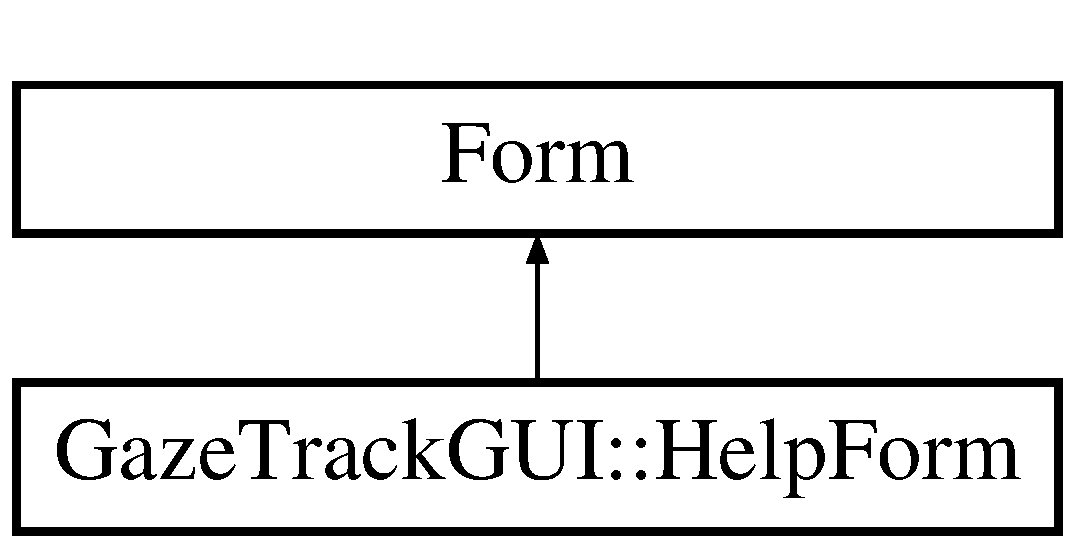
\includegraphics[height=2.000000cm]{class_gaze_track_g_u_i_1_1_help_form}
\end{center}
\end{figure}
\subsection*{Protected Member Functions}
\begin{DoxyCompactItemize}
\item 
\mbox{\hyperlink{class_gaze_track_g_u_i_1_1_help_form_a326e89f7265cbbd1b6070a143fa9fba4}{$\sim$\+Help\+Form}} ()
\begin{DoxyCompactList}\small\item\em Clean up any resources being used. \end{DoxyCompactList}\end{DoxyCompactItemize}
\subsection*{Private Member Functions}
\begin{DoxyCompactItemize}
\item 
void \mbox{\hyperlink{class_gaze_track_g_u_i_1_1_help_form_a00fee28d36e80735319d95098c26bbb2}{Initialize\+Component}} (void)
\begin{DoxyCompactList}\small\item\em Required method for Designer support -\/ do not modify the contents of this method with the code editor. \end{DoxyCompactList}\item 
\mbox{\Hypertarget{class_gaze_track_g_u_i_1_1_help_form_a1f45bc43ca6ea0dde9aea5752fda6f3e}\label{class_gaze_track_g_u_i_1_1_help_form_a1f45bc43ca6ea0dde9aea5752fda6f3e}} 
System\+::\+Void {\bfseries exit\+Btn\+\_\+\+Click} (System\+::\+Object$^\wedge$ sender, System\+::\+Event\+Args$^\wedge$ e)
\end{DoxyCompactItemize}
\subsection*{Private Attributes}
\begin{DoxyCompactItemize}
\item 
\mbox{\Hypertarget{class_gaze_track_g_u_i_1_1_help_form_aaa5fe087f4160afa36e1d80c74156579}\label{class_gaze_track_g_u_i_1_1_help_form_aaa5fe087f4160afa36e1d80c74156579}} 
System\+::\+Windows\+::\+Forms\+::\+Label $^\wedge$ {\bfseries label8}
\item 
\mbox{\Hypertarget{class_gaze_track_g_u_i_1_1_help_form_af9f13f8a629b767b341432a0030dfc36}\label{class_gaze_track_g_u_i_1_1_help_form_af9f13f8a629b767b341432a0030dfc36}} 
System\+::\+Windows\+::\+Forms\+::\+Button $^\wedge$ {\bfseries exit\+Btn}
\item 
\mbox{\Hypertarget{class_gaze_track_g_u_i_1_1_help_form_a2ff687bf84dcd326209d68a5dc8ce673}\label{class_gaze_track_g_u_i_1_1_help_form_a2ff687bf84dcd326209d68a5dc8ce673}} 
System\+::\+Windows\+::\+Forms\+::\+Rich\+Text\+Box $^\wedge$ {\bfseries rich\+Text\+Box6}
\item 
\mbox{\Hypertarget{class_gaze_track_g_u_i_1_1_help_form_abb74f4e40ef94f97daf50150e8258d44}\label{class_gaze_track_g_u_i_1_1_help_form_abb74f4e40ef94f97daf50150e8258d44}} 
System\+::\+Windows\+::\+Forms\+::\+Rich\+Text\+Box $^\wedge$ {\bfseries rich\+Text\+Box5}
\item 
\mbox{\Hypertarget{class_gaze_track_g_u_i_1_1_help_form_aa44193690ebc1131e73689534f6fe1cb}\label{class_gaze_track_g_u_i_1_1_help_form_aa44193690ebc1131e73689534f6fe1cb}} 
System\+::\+Windows\+::\+Forms\+::\+Rich\+Text\+Box $^\wedge$ {\bfseries rich\+Text\+Box4}
\item 
\mbox{\Hypertarget{class_gaze_track_g_u_i_1_1_help_form_ac6861c16d15c34ea73597909fce2bf8b}\label{class_gaze_track_g_u_i_1_1_help_form_ac6861c16d15c34ea73597909fce2bf8b}} 
System\+::\+Windows\+::\+Forms\+::\+Rich\+Text\+Box $^\wedge$ {\bfseries rich\+Text\+Box3}
\item 
\mbox{\Hypertarget{class_gaze_track_g_u_i_1_1_help_form_af44f180da06ea283ff05d016b3eb3949}\label{class_gaze_track_g_u_i_1_1_help_form_af44f180da06ea283ff05d016b3eb3949}} 
System\+::\+Windows\+::\+Forms\+::\+Rich\+Text\+Box $^\wedge$ {\bfseries rich\+Text\+Box2}
\item 
\mbox{\Hypertarget{class_gaze_track_g_u_i_1_1_help_form_a397095a0c72e317618fb249970caeda5}\label{class_gaze_track_g_u_i_1_1_help_form_a397095a0c72e317618fb249970caeda5}} 
System\+::\+Windows\+::\+Forms\+::\+Rich\+Text\+Box $^\wedge$ {\bfseries rich\+Text\+Box1}
\item 
\mbox{\Hypertarget{class_gaze_track_g_u_i_1_1_help_form_a22a3895c5164f46abe3e27ebdaab18f0}\label{class_gaze_track_g_u_i_1_1_help_form_a22a3895c5164f46abe3e27ebdaab18f0}} 
System\+::\+Windows\+::\+Forms\+::\+Label $^\wedge$ {\bfseries label7}
\item 
\mbox{\Hypertarget{class_gaze_track_g_u_i_1_1_help_form_a8f6eca8124302d3fc6548eb83e2423c4}\label{class_gaze_track_g_u_i_1_1_help_form_a8f6eca8124302d3fc6548eb83e2423c4}} 
System\+::\+Windows\+::\+Forms\+::\+Label $^\wedge$ {\bfseries label6}
\item 
\mbox{\Hypertarget{class_gaze_track_g_u_i_1_1_help_form_aa7cec3b7df9cfa3407ea6dded8d2453d}\label{class_gaze_track_g_u_i_1_1_help_form_aa7cec3b7df9cfa3407ea6dded8d2453d}} 
System\+::\+Windows\+::\+Forms\+::\+Label $^\wedge$ {\bfseries label5}
\item 
\mbox{\Hypertarget{class_gaze_track_g_u_i_1_1_help_form_ab766ec0d0531433aab577a5eaa021931}\label{class_gaze_track_g_u_i_1_1_help_form_ab766ec0d0531433aab577a5eaa021931}} 
System\+::\+Windows\+::\+Forms\+::\+Label $^\wedge$ {\bfseries label3}
\item 
\mbox{\Hypertarget{class_gaze_track_g_u_i_1_1_help_form_a210ac48f61d805a74914a7a48d70556f}\label{class_gaze_track_g_u_i_1_1_help_form_a210ac48f61d805a74914a7a48d70556f}} 
System\+::\+Windows\+::\+Forms\+::\+Label $^\wedge$ {\bfseries label2}
\item 
\mbox{\Hypertarget{class_gaze_track_g_u_i_1_1_help_form_a1916003b27ed300ab4d7a605aa591a61}\label{class_gaze_track_g_u_i_1_1_help_form_a1916003b27ed300ab4d7a605aa591a61}} 
System\+::\+Windows\+::\+Forms\+::\+Label $^\wedge$ {\bfseries label1}
\item 
System\+::\+Component\+Model\+::\+Container $^\wedge$ \mbox{\hyperlink{class_gaze_track_g_u_i_1_1_help_form_a562fda94d052719c80f2292dfd896f14}{components}}
\begin{DoxyCompactList}\small\item\em Required designer variable. \end{DoxyCompactList}\end{DoxyCompactItemize}


\subsection{Detailed Description}
Summary for \mbox{\hyperlink{class_gaze_track_g_u_i_1_1_help_form}{Help\+Form}} 



\subsection{Constructor \& Destructor Documentation}
\mbox{\Hypertarget{class_gaze_track_g_u_i_1_1_help_form_a326e89f7265cbbd1b6070a143fa9fba4}\label{class_gaze_track_g_u_i_1_1_help_form_a326e89f7265cbbd1b6070a143fa9fba4}} 
\index{Gaze\+Track\+G\+U\+I\+::\+Help\+Form@{Gaze\+Track\+G\+U\+I\+::\+Help\+Form}!````~Help\+Form@{$\sim$\+Help\+Form}}
\index{````~Help\+Form@{$\sim$\+Help\+Form}!Gaze\+Track\+G\+U\+I\+::\+Help\+Form@{Gaze\+Track\+G\+U\+I\+::\+Help\+Form}}
\subsubsection{\texorpdfstring{$\sim$\+Help\+Form()}{~HelpForm()}}
{\footnotesize\ttfamily Gaze\+Track\+G\+U\+I\+::\+Help\+Form\+::$\sim$\+Help\+Form (\begin{DoxyParamCaption}{ }\end{DoxyParamCaption})\hspace{0.3cm}{\ttfamily [inline]}, {\ttfamily [protected]}}



Clean up any resources being used. 



\subsection{Member Function Documentation}
\mbox{\Hypertarget{class_gaze_track_g_u_i_1_1_help_form_a00fee28d36e80735319d95098c26bbb2}\label{class_gaze_track_g_u_i_1_1_help_form_a00fee28d36e80735319d95098c26bbb2}} 
\index{Gaze\+Track\+G\+U\+I\+::\+Help\+Form@{Gaze\+Track\+G\+U\+I\+::\+Help\+Form}!Initialize\+Component@{Initialize\+Component}}
\index{Initialize\+Component@{Initialize\+Component}!Gaze\+Track\+G\+U\+I\+::\+Help\+Form@{Gaze\+Track\+G\+U\+I\+::\+Help\+Form}}
\subsubsection{\texorpdfstring{Initialize\+Component()}{InitializeComponent()}}
{\footnotesize\ttfamily void Gaze\+Track\+G\+U\+I\+::\+Help\+Form\+::\+Initialize\+Component (\begin{DoxyParamCaption}\item[{void}]{ }\end{DoxyParamCaption})\hspace{0.3cm}{\ttfamily [inline]}, {\ttfamily [private]}}



Required method for Designer support -\/ do not modify the contents of this method with the code editor. 



\subsection{Member Data Documentation}
\mbox{\Hypertarget{class_gaze_track_g_u_i_1_1_help_form_a562fda94d052719c80f2292dfd896f14}\label{class_gaze_track_g_u_i_1_1_help_form_a562fda94d052719c80f2292dfd896f14}} 
\index{Gaze\+Track\+G\+U\+I\+::\+Help\+Form@{Gaze\+Track\+G\+U\+I\+::\+Help\+Form}!components@{components}}
\index{components@{components}!Gaze\+Track\+G\+U\+I\+::\+Help\+Form@{Gaze\+Track\+G\+U\+I\+::\+Help\+Form}}
\subsubsection{\texorpdfstring{components}{components}}
{\footnotesize\ttfamily System\+::\+Component\+Model\+::\+Container $^\wedge$ Gaze\+Track\+G\+U\+I\+::\+Help\+Form\+::components\hspace{0.3cm}{\ttfamily [private]}}



Required designer variable. 



The documentation for this class was generated from the following file\+:\begin{DoxyCompactItemize}
\item 
F\+:/\+Gaze\+Track\+G\+U\+I/Help\+Form.\+h\end{DoxyCompactItemize}

\hypertarget{class_pupil_detect}{}\section{Pupil\+Detect Class Reference}
\label{class_pupil_detect}\index{Pupil\+Detect@{Pupil\+Detect}}
\subsection*{Public Member Functions}
\begin{DoxyCompactItemize}
\item 
\mbox{\hyperlink{class_pupil_detect_aa1ace17fac0af12bee24ca0413cc59a0}{Pupil\+Detect}} ()
\item 
\mbox{\hyperlink{struct_pupil_position}{Pupil\+Position}} \mbox{\hyperlink{class_pupil_detect_a95abbcaf36e31ea938ffdbc3402a481a}{get\+Pupil\+Position}} ()
\item 
\mbox{\hyperlink{struct_pupil_position}{Pupil\+Position}} $\ast$ \mbox{\hyperlink{class_pupil_detect_a41e24f18271f8395b1ab5043d70c03ad}{get\+Coordinates}} ()
\item 
\mbox{\hyperlink{struct_pupil_position}{Pupil\+Position}} \mbox{\hyperlink{class_pupil_detect_ae2338ef12da7fd0a0c2f668e25dbec54}{get\+Frame\+Dimensions}} ()
\item 
cv\+::\+Mat \mbox{\hyperlink{class_pupil_detect_a09f63f95f480233d90a648e0a61c8abb}{get\+Original\+Image}} (cv\+::\+Video\+Capture cap)
\item 
cv\+::\+Mat \mbox{\hyperlink{class_pupil_detect_af770df91c51d99bdd1a282e8b9fb6f1b}{get\+Processed\+Frame}} ()
\item 
void \mbox{\hyperlink{class_pupil_detect_aef0256a07774377932e949f2ba460fde}{init\+Calibration}} ()
\item 
void \mbox{\hyperlink{class_pupil_detect_a6c3419d438fde03cc460597257e05446}{detect\+Pupil}} (cv\+::\+Video\+Capture capture)
\item 
void \mbox{\hyperlink{class_pupil_detect_a59eaecc4b0dfb1c380d3c5d5ebf806f0}{set\+Video\+Status}} (bool \mbox{\hyperlink{class_pupil_detect_af956995e72f4c348ae4056aba2112e2b}{play}})
\item 
void \mbox{\hyperlink{class_pupil_detect_a22dc3e6f1496e1f0a79c61433f062cf0}{set\+Coordinates}} (int id)
\item 
void \mbox{\hyperlink{class_pupil_detect_ab1bc03f4007d91e575b349659119c70a}{find\+Eye}} ()
\item 
void \mbox{\hyperlink{class_pupil_detect_a116fb58487a120ee59642c6e97d77134}{set\+Threshold}} (int threshold\+In)
\item 
void \mbox{\hyperlink{class_pupil_detect_a38b91dc58b1a408e7ca081dac2c208bb}{set\+Max\+Area}} (int max\+Area\+In)
\item 
void \mbox{\hyperlink{class_pupil_detect_aa933cccabd0866e4fa1aee000532cb29}{set\+Min\+Area}} (int min\+Area\+In)
\item 
\mbox{\hyperlink{class_pupil_detect_af97e965d47623069188ffdf793248077}{$\sim$\+Pupil\+Detect}} ()
\end{DoxyCompactItemize}
\subsection*{Public Attributes}
\begin{DoxyCompactItemize}
\item 
\mbox{\Hypertarget{class_pupil_detect_a3aa92fd80cf4ae3084ec8a04ba7398a3}\label{class_pupil_detect_a3aa92fd80cf4ae3084ec8a04ba7398a3}} 
\mbox{\hyperlink{struct_pupil_position}{Pupil\+Position}} {\bfseries position}
\end{DoxyCompactItemize}
\subsection*{Private Member Functions}
\begin{DoxyCompactItemize}
\item 
void \mbox{\hyperlink{class_pupil_detect_ab852b491f3da3294e89d25777653e20f}{find\+Contours}} (cv\+::\+Mat \mbox{\hyperlink{class_pupil_detect_ad2b693a118fb991ea45cb8fb83dd0f63}{threshold\+Frame}})
\item 
void \mbox{\hyperlink{class_pupil_detect_a0ee35bec8dee73602288be1e95ab7b22}{apply\+Threshold}} (int thresh\+Hold\+Intensity)
\item 
void \mbox{\hyperlink{class_pupil_detect_aa1e4390aead747da32a2f1aaf077da68}{draw\+Contours}} (std\+::vector$<$ std\+::vector$<$ cv\+::\+Point $>$$>$ \mbox{\hyperlink{class_pupil_detect_a28325d88d52b09e78d25f17b3d898aeb}{contours}})
\end{DoxyCompactItemize}
\subsection*{Private Attributes}
\begin{DoxyCompactItemize}
\item 
cv\+::\+Mat \mbox{\hyperlink{class_pupil_detect_a2573a2415b451c876ab47a0ef016ec18}{current\+Frame}}
\item 
cv\+::\+Mat \mbox{\hyperlink{class_pupil_detect_ad2b693a118fb991ea45cb8fb83dd0f63}{threshold\+Frame}}
\item 
std\+::vector$<$ std\+::vector$<$ cv\+::\+Point $>$ $>$ \mbox{\hyperlink{class_pupil_detect_a28325d88d52b09e78d25f17b3d898aeb}{contours}}
\item 
std\+::vector$<$ cv\+::\+Rect $>$ \mbox{\hyperlink{class_pupil_detect_aee60f1bd292f20e41057139483c9d940}{eye}}
\item 
bool \mbox{\hyperlink{class_pupil_detect_af956995e72f4c348ae4056aba2112e2b}{play}}
\item 
int \mbox{\hyperlink{class_pupil_detect_a0a13ac6ad9894befc3da11ef02add74f}{threshold\+Intensity}}
\item 
int \mbox{\hyperlink{class_pupil_detect_a04fb7c5b3619d86b2f34ca90b56935e6}{max\+Area}}
\item 
int \mbox{\hyperlink{class_pupil_detect_ad1aa1a502f314a9dbdcfbb784cf14944}{min\+Area}}
\item 
int \mbox{\hyperlink{class_pupil_detect_a6fc0c70df2b083d7c24be0a4dff9d7a5}{counter}}
\item 
bool \mbox{\hyperlink{class_pupil_detect_ad4192b7bc071abfed746e463f383b866}{is\+Calibrating}}
\item 
double \mbox{\hyperlink{class_pupil_detect_a2649d7093083c33607bd412707773a51}{to\+Delay}}
\end{DoxyCompactItemize}


\subsection{Constructor \& Destructor Documentation}
\mbox{\Hypertarget{class_pupil_detect_aa1ace17fac0af12bee24ca0413cc59a0}\label{class_pupil_detect_aa1ace17fac0af12bee24ca0413cc59a0}} 
\index{Pupil\+Detect@{Pupil\+Detect}!Pupil\+Detect@{Pupil\+Detect}}
\index{Pupil\+Detect@{Pupil\+Detect}!Pupil\+Detect@{Pupil\+Detect}}
\subsubsection{\texorpdfstring{Pupil\+Detect()}{PupilDetect()}}
{\footnotesize\ttfamily Pupil\+Detect\+::\+Pupil\+Detect (\begin{DoxyParamCaption}{ }\end{DoxyParamCaption})}

Constructor of pupil Object \mbox{\Hypertarget{class_pupil_detect_af97e965d47623069188ffdf793248077}\label{class_pupil_detect_af97e965d47623069188ffdf793248077}} 
\index{Pupil\+Detect@{Pupil\+Detect}!````~Pupil\+Detect@{$\sim$\+Pupil\+Detect}}
\index{````~Pupil\+Detect@{$\sim$\+Pupil\+Detect}!Pupil\+Detect@{Pupil\+Detect}}
\subsubsection{\texorpdfstring{$\sim$\+Pupil\+Detect()}{~PupilDetect()}}
{\footnotesize\ttfamily Pupil\+Detect\+::$\sim$\+Pupil\+Detect (\begin{DoxyParamCaption}{ }\end{DoxyParamCaption})}

\mbox{\hyperlink{class_pupil_detect}{Pupil\+Detect}} Object destructor 

\subsection{Member Function Documentation}
\mbox{\Hypertarget{class_pupil_detect_a0ee35bec8dee73602288be1e95ab7b22}\label{class_pupil_detect_a0ee35bec8dee73602288be1e95ab7b22}} 
\index{Pupil\+Detect@{Pupil\+Detect}!apply\+Threshold@{apply\+Threshold}}
\index{apply\+Threshold@{apply\+Threshold}!Pupil\+Detect@{Pupil\+Detect}}
\subsubsection{\texorpdfstring{apply\+Threshold()}{applyThreshold()}}
{\footnotesize\ttfamily void Pupil\+Detect\+::apply\+Threshold (\begin{DoxyParamCaption}\item[{int}]{thresh\+Hold\+Intensity }\end{DoxyParamCaption})\hspace{0.3cm}{\ttfamily [private]}}

Applies desired threshold to current frame \mbox{\Hypertarget{class_pupil_detect_a6c3419d438fde03cc460597257e05446}\label{class_pupil_detect_a6c3419d438fde03cc460597257e05446}} 
\index{Pupil\+Detect@{Pupil\+Detect}!detect\+Pupil@{detect\+Pupil}}
\index{detect\+Pupil@{detect\+Pupil}!Pupil\+Detect@{Pupil\+Detect}}
\subsubsection{\texorpdfstring{detect\+Pupil()}{detectPupil()}}
{\footnotesize\ttfamily void Pupil\+Detect\+::detect\+Pupil (\begin{DoxyParamCaption}\item[{cv\+::\+Video\+Capture}]{capture }\end{DoxyParamCaption})}

Puts together all funcitons in order to detect pupil \mbox{\Hypertarget{class_pupil_detect_aa1e4390aead747da32a2f1aaf077da68}\label{class_pupil_detect_aa1e4390aead747da32a2f1aaf077da68}} 
\index{Pupil\+Detect@{Pupil\+Detect}!draw\+Contours@{draw\+Contours}}
\index{draw\+Contours@{draw\+Contours}!Pupil\+Detect@{Pupil\+Detect}}
\subsubsection{\texorpdfstring{draw\+Contours()}{drawContours()}}
{\footnotesize\ttfamily void Pupil\+Detect\+::draw\+Contours (\begin{DoxyParamCaption}\item[{std\+::vector$<$ std\+::vector$<$ cv\+::\+Point $>$$>$}]{contours }\end{DoxyParamCaption})\hspace{0.3cm}{\ttfamily [private]}}

Draws the contours onto the frame for debugging purposes To find the center of each contour it finds their center of masses first Also draw the points acquired during calibration \mbox{\Hypertarget{class_pupil_detect_ab852b491f3da3294e89d25777653e20f}\label{class_pupil_detect_ab852b491f3da3294e89d25777653e20f}} 
\index{Pupil\+Detect@{Pupil\+Detect}!find\+Contours@{find\+Contours}}
\index{find\+Contours@{find\+Contours}!Pupil\+Detect@{Pupil\+Detect}}
\subsubsection{\texorpdfstring{find\+Contours()}{findContours()}}
{\footnotesize\ttfamily void Pupil\+Detect\+::find\+Contours (\begin{DoxyParamCaption}\item[{cv\+::\+Mat}]{threshold\+Frame }\end{DoxyParamCaption})\hspace{0.3cm}{\ttfamily [private]}}

Finds the contours in current frame and stores them in a vector object \mbox{\Hypertarget{class_pupil_detect_ab1bc03f4007d91e575b349659119c70a}\label{class_pupil_detect_ab1bc03f4007d91e575b349659119c70a}} 
\index{Pupil\+Detect@{Pupil\+Detect}!find\+Eye@{find\+Eye}}
\index{find\+Eye@{find\+Eye}!Pupil\+Detect@{Pupil\+Detect}}
\subsubsection{\texorpdfstring{find\+Eye()}{findEye()}}
{\footnotesize\ttfamily void Pupil\+Detect\+::find\+Eye (\begin{DoxyParamCaption}{ }\end{DoxyParamCaption})}

Isolate the region where eye is detected \mbox{\Hypertarget{class_pupil_detect_a41e24f18271f8395b1ab5043d70c03ad}\label{class_pupil_detect_a41e24f18271f8395b1ab5043d70c03ad}} 
\index{Pupil\+Detect@{Pupil\+Detect}!get\+Coordinates@{get\+Coordinates}}
\index{get\+Coordinates@{get\+Coordinates}!Pupil\+Detect@{Pupil\+Detect}}
\subsubsection{\texorpdfstring{get\+Coordinates()}{getCoordinates()}}
{\footnotesize\ttfamily \mbox{\hyperlink{struct_pupil_position}{Pupil\+Position}} $\ast$ Pupil\+Detect\+::get\+Coordinates (\begin{DoxyParamCaption}{ }\end{DoxyParamCaption})}

Gets the array of coordinates acquired during calibration \mbox{\Hypertarget{class_pupil_detect_ae2338ef12da7fd0a0c2f668e25dbec54}\label{class_pupil_detect_ae2338ef12da7fd0a0c2f668e25dbec54}} 
\index{Pupil\+Detect@{Pupil\+Detect}!get\+Frame\+Dimensions@{get\+Frame\+Dimensions}}
\index{get\+Frame\+Dimensions@{get\+Frame\+Dimensions}!Pupil\+Detect@{Pupil\+Detect}}
\subsubsection{\texorpdfstring{get\+Frame\+Dimensions()}{getFrameDimensions()}}
{\footnotesize\ttfamily \mbox{\hyperlink{struct_pupil_position}{Pupil\+Position}} Pupil\+Detect\+::get\+Frame\+Dimensions (\begin{DoxyParamCaption}{ }\end{DoxyParamCaption})}

Gets the width and height or the camera frame \mbox{\Hypertarget{class_pupil_detect_a09f63f95f480233d90a648e0a61c8abb}\label{class_pupil_detect_a09f63f95f480233d90a648e0a61c8abb}} 
\index{Pupil\+Detect@{Pupil\+Detect}!get\+Original\+Image@{get\+Original\+Image}}
\index{get\+Original\+Image@{get\+Original\+Image}!Pupil\+Detect@{Pupil\+Detect}}
\subsubsection{\texorpdfstring{get\+Original\+Image()}{getOriginalImage()}}
{\footnotesize\ttfamily cv\+::\+Mat Pupil\+Detect\+::get\+Original\+Image (\begin{DoxyParamCaption}\item[{cv\+::\+Video\+Capture}]{cap }\end{DoxyParamCaption})}

Reads the image from camera \mbox{\Hypertarget{class_pupil_detect_af770df91c51d99bdd1a282e8b9fb6f1b}\label{class_pupil_detect_af770df91c51d99bdd1a282e8b9fb6f1b}} 
\index{Pupil\+Detect@{Pupil\+Detect}!get\+Processed\+Frame@{get\+Processed\+Frame}}
\index{get\+Processed\+Frame@{get\+Processed\+Frame}!Pupil\+Detect@{Pupil\+Detect}}
\subsubsection{\texorpdfstring{get\+Processed\+Frame()}{getProcessedFrame()}}
{\footnotesize\ttfamily cv\+::\+Mat Pupil\+Detect\+::get\+Processed\+Frame (\begin{DoxyParamCaption}{ }\end{DoxyParamCaption})}

Returns a frame after a pupil has been found \mbox{\Hypertarget{class_pupil_detect_a95abbcaf36e31ea938ffdbc3402a481a}\label{class_pupil_detect_a95abbcaf36e31ea938ffdbc3402a481a}} 
\index{Pupil\+Detect@{Pupil\+Detect}!get\+Pupil\+Position@{get\+Pupil\+Position}}
\index{get\+Pupil\+Position@{get\+Pupil\+Position}!Pupil\+Detect@{Pupil\+Detect}}
\subsubsection{\texorpdfstring{get\+Pupil\+Position()}{getPupilPosition()}}
{\footnotesize\ttfamily \mbox{\hyperlink{struct_pupil_position}{Pupil\+Position}} Pupil\+Detect\+::get\+Pupil\+Position (\begin{DoxyParamCaption}{ }\end{DoxyParamCaption})}

Returns current coordinates of the pupil \mbox{\Hypertarget{class_pupil_detect_aef0256a07774377932e949f2ba460fde}\label{class_pupil_detect_aef0256a07774377932e949f2ba460fde}} 
\index{Pupil\+Detect@{Pupil\+Detect}!init\+Calibration@{init\+Calibration}}
\index{init\+Calibration@{init\+Calibration}!Pupil\+Detect@{Pupil\+Detect}}
\subsubsection{\texorpdfstring{init\+Calibration()}{initCalibration()}}
{\footnotesize\ttfamily void Pupil\+Detect\+::init\+Calibration (\begin{DoxyParamCaption}{ }\end{DoxyParamCaption})}

Determines if the program is in calibration phase \mbox{\Hypertarget{class_pupil_detect_a22dc3e6f1496e1f0a79c61433f062cf0}\label{class_pupil_detect_a22dc3e6f1496e1f0a79c61433f062cf0}} 
\index{Pupil\+Detect@{Pupil\+Detect}!set\+Coordinates@{set\+Coordinates}}
\index{set\+Coordinates@{set\+Coordinates}!Pupil\+Detect@{Pupil\+Detect}}
\subsubsection{\texorpdfstring{set\+Coordinates()}{setCoordinates()}}
{\footnotesize\ttfamily void Pupil\+Detect\+::set\+Coordinates (\begin{DoxyParamCaption}\item[{int}]{id }\end{DoxyParamCaption})}

Gets the pupil cordinates from calibration form and stores them id is the identifiers of a calibration point or a button \mbox{\Hypertarget{class_pupil_detect_a38b91dc58b1a408e7ca081dac2c208bb}\label{class_pupil_detect_a38b91dc58b1a408e7ca081dac2c208bb}} 
\index{Pupil\+Detect@{Pupil\+Detect}!set\+Max\+Area@{set\+Max\+Area}}
\index{set\+Max\+Area@{set\+Max\+Area}!Pupil\+Detect@{Pupil\+Detect}}
\subsubsection{\texorpdfstring{set\+Max\+Area()}{setMaxArea()}}
{\footnotesize\ttfamily void Pupil\+Detect\+::set\+Max\+Area (\begin{DoxyParamCaption}\item[{int}]{max\+Area\+In }\end{DoxyParamCaption})}

Gets new value from maximum area slider in the main G\+UI 
\begin{DoxyParams}{Parameters}
{\em max\+Area\+In} & The value that is to set as maximum \\
\hline
\end{DoxyParams}
\mbox{\Hypertarget{class_pupil_detect_aa933cccabd0866e4fa1aee000532cb29}\label{class_pupil_detect_aa933cccabd0866e4fa1aee000532cb29}} 
\index{Pupil\+Detect@{Pupil\+Detect}!set\+Min\+Area@{set\+Min\+Area}}
\index{set\+Min\+Area@{set\+Min\+Area}!Pupil\+Detect@{Pupil\+Detect}}
\subsubsection{\texorpdfstring{set\+Min\+Area()}{setMinArea()}}
{\footnotesize\ttfamily void Pupil\+Detect\+::set\+Min\+Area (\begin{DoxyParamCaption}\item[{int}]{min\+Area\+In }\end{DoxyParamCaption})}

Gets new value from minimum area slider in the main G\+UI 
\begin{DoxyParams}{Parameters}
{\em min\+Area\+In} & The value that is to set as maximum \\
\hline
\end{DoxyParams}
\mbox{\Hypertarget{class_pupil_detect_a116fb58487a120ee59642c6e97d77134}\label{class_pupil_detect_a116fb58487a120ee59642c6e97d77134}} 
\index{Pupil\+Detect@{Pupil\+Detect}!set\+Threshold@{set\+Threshold}}
\index{set\+Threshold@{set\+Threshold}!Pupil\+Detect@{Pupil\+Detect}}
\subsubsection{\texorpdfstring{set\+Threshold()}{setThreshold()}}
{\footnotesize\ttfamily void Pupil\+Detect\+::set\+Threshold (\begin{DoxyParamCaption}\item[{int}]{threshold\+In }\end{DoxyParamCaption})}

Gets new value from threshold slider in the main G\+UI \mbox{\Hypertarget{class_pupil_detect_a59eaecc4b0dfb1c380d3c5d5ebf806f0}\label{class_pupil_detect_a59eaecc4b0dfb1c380d3c5d5ebf806f0}} 
\index{Pupil\+Detect@{Pupil\+Detect}!set\+Video\+Status@{set\+Video\+Status}}
\index{set\+Video\+Status@{set\+Video\+Status}!Pupil\+Detect@{Pupil\+Detect}}
\subsubsection{\texorpdfstring{set\+Video\+Status()}{setVideoStatus()}}
{\footnotesize\ttfamily void Pupil\+Detect\+::set\+Video\+Status (\begin{DoxyParamCaption}\item[{bool}]{play\+In }\end{DoxyParamCaption})}

Stops video capture when the main program has been stopped 
\begin{DoxyParams}{Parameters}
{\em play\+In} & A boolean to decide if video should play or not \\
\hline
\end{DoxyParams}


\subsection{Member Data Documentation}
\mbox{\Hypertarget{class_pupil_detect_a28325d88d52b09e78d25f17b3d898aeb}\label{class_pupil_detect_a28325d88d52b09e78d25f17b3d898aeb}} 
\index{Pupil\+Detect@{Pupil\+Detect}!contours@{contours}}
\index{contours@{contours}!Pupil\+Detect@{Pupil\+Detect}}
\subsubsection{\texorpdfstring{contours}{contours}}
{\footnotesize\ttfamily std\+::vector$<$std\+::vector$<$cv\+::\+Point$>$ $>$ Pupil\+Detect\+::contours\hspace{0.3cm}{\ttfamily [private]}}

1D vector which contains all the contours in a threshold frame \mbox{\Hypertarget{class_pupil_detect_a6fc0c70df2b083d7c24be0a4dff9d7a5}\label{class_pupil_detect_a6fc0c70df2b083d7c24be0a4dff9d7a5}} 
\index{Pupil\+Detect@{Pupil\+Detect}!counter@{counter}}
\index{counter@{counter}!Pupil\+Detect@{Pupil\+Detect}}
\subsubsection{\texorpdfstring{counter}{counter}}
{\footnotesize\ttfamily int Pupil\+Detect\+::counter\hspace{0.3cm}{\ttfamily [private]}}

Counts number of points that are aready calibrated \mbox{\Hypertarget{class_pupil_detect_a2573a2415b451c876ab47a0ef016ec18}\label{class_pupil_detect_a2573a2415b451c876ab47a0ef016ec18}} 
\index{Pupil\+Detect@{Pupil\+Detect}!current\+Frame@{current\+Frame}}
\index{current\+Frame@{current\+Frame}!Pupil\+Detect@{Pupil\+Detect}}
\subsubsection{\texorpdfstring{current\+Frame}{currentFrame}}
{\footnotesize\ttfamily cv\+::\+Mat Pupil\+Detect\+::current\+Frame\hspace{0.3cm}{\ttfamily [private]}}

Current frame that is being processed \mbox{\Hypertarget{class_pupil_detect_aee60f1bd292f20e41057139483c9d940}\label{class_pupil_detect_aee60f1bd292f20e41057139483c9d940}} 
\index{Pupil\+Detect@{Pupil\+Detect}!eye@{eye}}
\index{eye@{eye}!Pupil\+Detect@{Pupil\+Detect}}
\subsubsection{\texorpdfstring{eye}{eye}}
{\footnotesize\ttfamily std\+::vector$<$cv\+::\+Rect$>$ Pupil\+Detect\+::eye\hspace{0.3cm}{\ttfamily [private]}}

1D vector of rectangles where eye can be potentially found \mbox{\Hypertarget{class_pupil_detect_ad4192b7bc071abfed746e463f383b866}\label{class_pupil_detect_ad4192b7bc071abfed746e463f383b866}} 
\index{Pupil\+Detect@{Pupil\+Detect}!is\+Calibrating@{is\+Calibrating}}
\index{is\+Calibrating@{is\+Calibrating}!Pupil\+Detect@{Pupil\+Detect}}
\subsubsection{\texorpdfstring{is\+Calibrating}{isCalibrating}}
{\footnotesize\ttfamily bool Pupil\+Detect\+::is\+Calibrating\hspace{0.3cm}{\ttfamily [private]}}

Defines if the user is calibrating or not \mbox{\Hypertarget{class_pupil_detect_a04fb7c5b3619d86b2f34ca90b56935e6}\label{class_pupil_detect_a04fb7c5b3619d86b2f34ca90b56935e6}} 
\index{Pupil\+Detect@{Pupil\+Detect}!max\+Area@{max\+Area}}
\index{max\+Area@{max\+Area}!Pupil\+Detect@{Pupil\+Detect}}
\subsubsection{\texorpdfstring{max\+Area}{maxArea}}
{\footnotesize\ttfamily int Pupil\+Detect\+::max\+Area\hspace{0.3cm}{\ttfamily [private]}}

Variable maximum logical area for a contour to be a pupil \mbox{\Hypertarget{class_pupil_detect_ad1aa1a502f314a9dbdcfbb784cf14944}\label{class_pupil_detect_ad1aa1a502f314a9dbdcfbb784cf14944}} 
\index{Pupil\+Detect@{Pupil\+Detect}!min\+Area@{min\+Area}}
\index{min\+Area@{min\+Area}!Pupil\+Detect@{Pupil\+Detect}}
\subsubsection{\texorpdfstring{min\+Area}{minArea}}
{\footnotesize\ttfamily int Pupil\+Detect\+::min\+Area\hspace{0.3cm}{\ttfamily [private]}}

Variable minimum logical area for a contour to be a pupil \mbox{\Hypertarget{class_pupil_detect_af956995e72f4c348ae4056aba2112e2b}\label{class_pupil_detect_af956995e72f4c348ae4056aba2112e2b}} 
\index{Pupil\+Detect@{Pupil\+Detect}!play@{play}}
\index{play@{play}!Pupil\+Detect@{Pupil\+Detect}}
\subsubsection{\texorpdfstring{play}{play}}
{\footnotesize\ttfamily bool Pupil\+Detect\+::play\hspace{0.3cm}{\ttfamily [private]}}

This is used to play or pause the video from camera \mbox{\Hypertarget{class_pupil_detect_ad2b693a118fb991ea45cb8fb83dd0f63}\label{class_pupil_detect_ad2b693a118fb991ea45cb8fb83dd0f63}} 
\index{Pupil\+Detect@{Pupil\+Detect}!threshold\+Frame@{threshold\+Frame}}
\index{threshold\+Frame@{threshold\+Frame}!Pupil\+Detect@{Pupil\+Detect}}
\subsubsection{\texorpdfstring{threshold\+Frame}{thresholdFrame}}
{\footnotesize\ttfamily cv\+::\+Mat Pupil\+Detect\+::threshold\+Frame\hspace{0.3cm}{\ttfamily [private]}}

Current frame after applying threshold \mbox{\Hypertarget{class_pupil_detect_a0a13ac6ad9894befc3da11ef02add74f}\label{class_pupil_detect_a0a13ac6ad9894befc3da11ef02add74f}} 
\index{Pupil\+Detect@{Pupil\+Detect}!threshold\+Intensity@{threshold\+Intensity}}
\index{threshold\+Intensity@{threshold\+Intensity}!Pupil\+Detect@{Pupil\+Detect}}
\subsubsection{\texorpdfstring{threshold\+Intensity}{thresholdIntensity}}
{\footnotesize\ttfamily int Pupil\+Detect\+::threshold\+Intensity\hspace{0.3cm}{\ttfamily [private]}}

Variable intensity for a camera frame \mbox{\Hypertarget{class_pupil_detect_a2649d7093083c33607bd412707773a51}\label{class_pupil_detect_a2649d7093083c33607bd412707773a51}} 
\index{Pupil\+Detect@{Pupil\+Detect}!to\+Delay@{to\+Delay}}
\index{to\+Delay@{to\+Delay}!Pupil\+Detect@{Pupil\+Detect}}
\subsubsection{\texorpdfstring{to\+Delay}{toDelay}}
{\footnotesize\ttfamily double Pupil\+Detect\+::to\+Delay\hspace{0.3cm}{\ttfamily [private]}}

Delay input from user to avoid quick presses of a button 

The documentation for this class was generated from the following files\+:\begin{DoxyCompactItemize}
\item 
F\+:/\+Gaze\+Track\+G\+U\+I/Pupil\+Detect.\+h\item 
F\+:/\+Gaze\+Track\+G\+U\+I/Pupil\+Detect.\+cpp\end{DoxyCompactItemize}

\hypertarget{struct_pupil_position}{}\section{Pupil\+Position Struct Reference}
\label{struct_pupil_position}\index{Pupil\+Position@{Pupil\+Position}}


{\ttfamily \#include $<$Pupil\+Detect.\+h$>$}

\subsection*{Public Attributes}
\begin{DoxyCompactItemize}
\item 
\mbox{\Hypertarget{struct_pupil_position_a2e46ffc2d7349801767dc4ed827d9ab0}\label{struct_pupil_position_a2e46ffc2d7349801767dc4ed827d9ab0}} 
int {\bfseries x}
\item 
\mbox{\Hypertarget{struct_pupil_position_a9b676752799afa74e780f1beb206c97c}\label{struct_pupil_position_a9b676752799afa74e780f1beb206c97c}} 
int {\bfseries y}
\end{DoxyCompactItemize}


\subsection{Detailed Description}
A Struct for position the pupil 
\begin{DoxyParams}{Parameters}
{\em x,y} & Coordinates of a point \\
\hline
\end{DoxyParams}


The documentation for this struct was generated from the following file\+:\begin{DoxyCompactItemize}
\item 
F\+:/\+Gaze\+Track\+G\+U\+I/Pupil\+Detect.\+h\end{DoxyCompactItemize}

\hypertarget{class_gaze_track_g_u_i_1_1_tester}{}\section{Gaze\+Track\+G\+UI\+:\+:Tester Class Reference}
\label{class_gaze_track_g_u_i_1_1_tester}\index{Gaze\+Track\+G\+U\+I\+::\+Tester@{Gaze\+Track\+G\+U\+I\+::\+Tester}}


Summary for \mbox{\hyperlink{class_gaze_track_g_u_i_1_1_tester}{Tester}}  




{\ttfamily \#include $<$Tester.\+h$>$}

Inheritance diagram for Gaze\+Track\+G\+UI\+:\+:Tester\+:\begin{figure}[H]
\begin{center}
\leavevmode
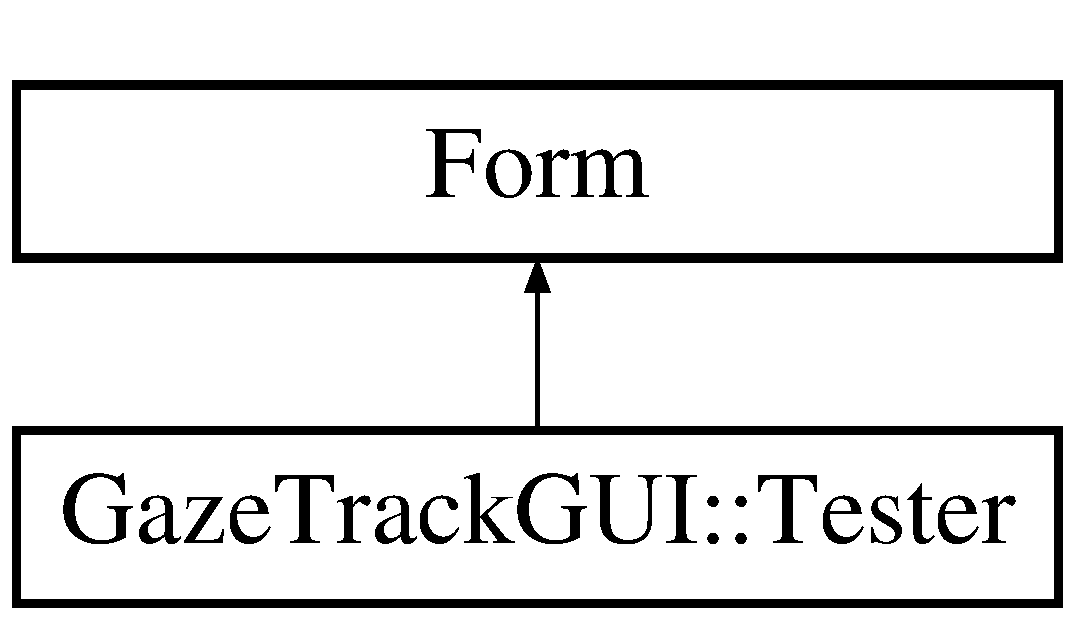
\includegraphics[height=2.000000cm]{class_gaze_track_g_u_i_1_1_tester}
\end{center}
\end{figure}
\subsection*{Public Attributes}
\begin{DoxyCompactItemize}
\item 
\mbox{\Hypertarget{class_gaze_track_g_u_i_1_1_tester_a6d7e79e27e3dd658636b5e9c63b549d2}\label{class_gaze_track_g_u_i_1_1_tester_a6d7e79e27e3dd658636b5e9c63b549d2}} 
int {\bfseries counter1} = 5
\end{DoxyCompactItemize}
\subsection*{Protected Member Functions}
\begin{DoxyCompactItemize}
\item 
\mbox{\hyperlink{class_gaze_track_g_u_i_1_1_tester_ac42ed2ea3e4c5b2fbdafe6d11d26cb49}{$\sim$\+Tester}} ()
\begin{DoxyCompactList}\small\item\em Clean up any resources being used. \end{DoxyCompactList}\end{DoxyCompactItemize}
\subsection*{Private Member Functions}
\begin{DoxyCompactItemize}
\item 
int \mbox{\hyperlink{class_gaze_track_g_u_i_1_1_tester_a76eaf835618462a5a78858946a0c8f12}{generate\+RandomX}} ()
\item 
int \mbox{\hyperlink{class_gaze_track_g_u_i_1_1_tester_af67ef1c7ec226026dfb05f2d7fb8245e}{generate\+RandomY}} ()
\item 
void \mbox{\hyperlink{class_gaze_track_g_u_i_1_1_tester_a5d43b09e8e58ab48a5299fabbdb075a6}{move\+Image\+Box}} ()
\item 
void \mbox{\hyperlink{class_gaze_track_g_u_i_1_1_tester_abbfdda1b0d394b72af518d259b150d75}{calculate\+Distance}} ()
\item 
void \mbox{\hyperlink{class_gaze_track_g_u_i_1_1_tester_a18f3d904b9d5a2faffb6c2ef4c5c58a3}{Initialize\+Component}} (void)
\begin{DoxyCompactList}\small\item\em Required designer variable. \end{DoxyCompactList}\item 
\mbox{\Hypertarget{class_gaze_track_g_u_i_1_1_tester_ae594801ae74283c48436306e8b8b7031}\label{class_gaze_track_g_u_i_1_1_tester_ae594801ae74283c48436306e8b8b7031}} 
System\+::\+Void {\bfseries Tester\+\_\+\+Load} (System\+::\+Object$^\wedge$ sender, System\+::\+Event\+Args$^\wedge$ e)
\item 
\mbox{\Hypertarget{class_gaze_track_g_u_i_1_1_tester_a9a1be2fe47795bd37496e9e9d6ebc6ca}\label{class_gaze_track_g_u_i_1_1_tester_a9a1be2fe47795bd37496e9e9d6ebc6ca}} 
System\+::\+Void {\bfseries exit\+Button\+\_\+\+Click} (System\+::\+Object$^\wedge$ sender, System\+::\+Event\+Args$^\wedge$ e)
\item 
\mbox{\Hypertarget{class_gaze_track_g_u_i_1_1_tester_a3629cfa07ca8b4b8c79728d0108720b6}\label{class_gaze_track_g_u_i_1_1_tester_a3629cfa07ca8b4b8c79728d0108720b6}} 
System\+::\+Void {\bfseries generator\+Timer\+\_\+\+Tick} (System\+::\+Object$^\wedge$ sender, System\+::\+Event\+Args$^\wedge$ e)
\item 
\mbox{\Hypertarget{class_gaze_track_g_u_i_1_1_tester_afc18ba67318982c438251bb83239cb13}\label{class_gaze_track_g_u_i_1_1_tester_afc18ba67318982c438251bb83239cb13}} 
System\+::\+Void {\bfseries countdown\+Timer\+\_\+\+Tick} (System\+::\+Object$^\wedge$ sender, System\+::\+Event\+Args$^\wedge$ e)
\item 
\mbox{\Hypertarget{class_gaze_track_g_u_i_1_1_tester_a2ffc817b5ca0f066dcc648e156029b3e}\label{class_gaze_track_g_u_i_1_1_tester_a2ffc817b5ca0f066dcc648e156029b3e}} 
System\+::\+Void {\bfseries Tester\+\_\+\+Form\+Closed} (System\+::\+Object$^\wedge$ sender, System\+::\+Windows\+::\+Forms\+::\+Form\+Closed\+Event\+Args$^\wedge$ e)
\end{DoxyCompactItemize}
\subsection*{Private Attributes}
\begin{DoxyCompactItemize}
\item 
\mbox{\Hypertarget{class_gaze_track_g_u_i_1_1_tester_ad8ab6cca206f013af0205fd7326427cc}\label{class_gaze_track_g_u_i_1_1_tester_ad8ab6cca206f013af0205fd7326427cc}} 
System\+::\+Windows\+::\+Forms\+::\+Button $^\wedge$ {\bfseries exit\+Button}
\item 
\mbox{\Hypertarget{class_gaze_track_g_u_i_1_1_tester_a94dbcde5404ca0a61b9d8d3d1db7d241}\label{class_gaze_track_g_u_i_1_1_tester_a94dbcde5404ca0a61b9d8d3d1db7d241}} 
System\+::\+Windows\+::\+Forms\+::\+Picture\+Box $^\wedge$ {\bfseries img\+Box}
\item 
\mbox{\Hypertarget{class_gaze_track_g_u_i_1_1_tester_a6913d8af3a41d24b387d429edbe6d910}\label{class_gaze_track_g_u_i_1_1_tester_a6913d8af3a41d24b387d429edbe6d910}} 
System\+::\+Windows\+::\+Forms\+::\+Timer $^\wedge$ {\bfseries generator\+Timer}
\item 
\mbox{\Hypertarget{class_gaze_track_g_u_i_1_1_tester_a72f511e24714c8fdef4cd1fec72299eb}\label{class_gaze_track_g_u_i_1_1_tester_a72f511e24714c8fdef4cd1fec72299eb}} 
System\+::\+Windows\+::\+Forms\+::\+Timer $^\wedge$ {\bfseries countdown\+Timer}
\item 
\mbox{\Hypertarget{class_gaze_track_g_u_i_1_1_tester_af75f068e6faa57091d470f22bab03398}\label{class_gaze_track_g_u_i_1_1_tester_af75f068e6faa57091d470f22bab03398}} 
System\+::\+Windows\+::\+Forms\+::\+Label $^\wedge$ {\bfseries count\+Lbl}
\item 
\mbox{\Hypertarget{class_gaze_track_g_u_i_1_1_tester_a1104a0fbf9f3d6afe8132c29a4bc8ef7}\label{class_gaze_track_g_u_i_1_1_tester_a1104a0fbf9f3d6afe8132c29a4bc8ef7}} 
System\+::\+Component\+Model\+::\+I\+Container $^\wedge$ {\bfseries components}
\item 
\mbox{\Hypertarget{class_gaze_track_g_u_i_1_1_tester_a8082911a9e1adf4545844f1812161546}\label{class_gaze_track_g_u_i_1_1_tester_a8082911a9e1adf4545844f1812161546}} 
Point {\bfseries cursor\+Pos}
\end{DoxyCompactItemize}


\subsection{Detailed Description}
Summary for \mbox{\hyperlink{class_gaze_track_g_u_i_1_1_tester}{Tester}} 



\subsection{Constructor \& Destructor Documentation}
\mbox{\Hypertarget{class_gaze_track_g_u_i_1_1_tester_ac42ed2ea3e4c5b2fbdafe6d11d26cb49}\label{class_gaze_track_g_u_i_1_1_tester_ac42ed2ea3e4c5b2fbdafe6d11d26cb49}} 
\index{Gaze\+Track\+G\+U\+I\+::\+Tester@{Gaze\+Track\+G\+U\+I\+::\+Tester}!````~Tester@{$\sim$\+Tester}}
\index{````~Tester@{$\sim$\+Tester}!Gaze\+Track\+G\+U\+I\+::\+Tester@{Gaze\+Track\+G\+U\+I\+::\+Tester}}
\subsubsection{\texorpdfstring{$\sim$\+Tester()}{~Tester()}}
{\footnotesize\ttfamily Gaze\+Track\+G\+U\+I\+::\+Tester\+::$\sim$\+Tester (\begin{DoxyParamCaption}{ }\end{DoxyParamCaption})\hspace{0.3cm}{\ttfamily [inline]}, {\ttfamily [protected]}}



Clean up any resources being used. 



\subsection{Member Function Documentation}
\mbox{\Hypertarget{class_gaze_track_g_u_i_1_1_tester_abbfdda1b0d394b72af518d259b150d75}\label{class_gaze_track_g_u_i_1_1_tester_abbfdda1b0d394b72af518d259b150d75}} 
\index{Gaze\+Track\+G\+U\+I\+::\+Tester@{Gaze\+Track\+G\+U\+I\+::\+Tester}!calculate\+Distance@{calculate\+Distance}}
\index{calculate\+Distance@{calculate\+Distance}!Gaze\+Track\+G\+U\+I\+::\+Tester@{Gaze\+Track\+G\+U\+I\+::\+Tester}}
\subsubsection{\texorpdfstring{calculate\+Distance()}{calculateDistance()}}
{\footnotesize\ttfamily void Gaze\+Track\+G\+U\+I\+::\+Tester\+::calculate\+Distance (\begin{DoxyParamCaption}{ }\end{DoxyParamCaption})\hspace{0.3cm}{\ttfamily [private]}}

Calculates distance between the coordinates of the image/circle and coordinates of the cursor/mouse pointer Writes this distance to a file \mbox{\Hypertarget{class_gaze_track_g_u_i_1_1_tester_a76eaf835618462a5a78858946a0c8f12}\label{class_gaze_track_g_u_i_1_1_tester_a76eaf835618462a5a78858946a0c8f12}} 
\index{Gaze\+Track\+G\+U\+I\+::\+Tester@{Gaze\+Track\+G\+U\+I\+::\+Tester}!generate\+RandomX@{generate\+RandomX}}
\index{generate\+RandomX@{generate\+RandomX}!Gaze\+Track\+G\+U\+I\+::\+Tester@{Gaze\+Track\+G\+U\+I\+::\+Tester}}
\subsubsection{\texorpdfstring{generate\+Random\+X()}{generateRandomX()}}
{\footnotesize\ttfamily int Gaze\+Track\+G\+U\+I\+::\+Tester\+::generate\+RandomX (\begin{DoxyParamCaption}{ }\end{DoxyParamCaption})\hspace{0.3cm}{\ttfamily [private]}}

Generates a random X coordinate where the circle would be placed \mbox{\Hypertarget{class_gaze_track_g_u_i_1_1_tester_af67ef1c7ec226026dfb05f2d7fb8245e}\label{class_gaze_track_g_u_i_1_1_tester_af67ef1c7ec226026dfb05f2d7fb8245e}} 
\index{Gaze\+Track\+G\+U\+I\+::\+Tester@{Gaze\+Track\+G\+U\+I\+::\+Tester}!generate\+RandomY@{generate\+RandomY}}
\index{generate\+RandomY@{generate\+RandomY}!Gaze\+Track\+G\+U\+I\+::\+Tester@{Gaze\+Track\+G\+U\+I\+::\+Tester}}
\subsubsection{\texorpdfstring{generate\+Random\+Y()}{generateRandomY()}}
{\footnotesize\ttfamily int Gaze\+Track\+G\+U\+I\+::\+Tester\+::generate\+RandomY (\begin{DoxyParamCaption}{ }\end{DoxyParamCaption})\hspace{0.3cm}{\ttfamily [private]}}

Generates a random Y coordinate where the circle would be placed \mbox{\Hypertarget{class_gaze_track_g_u_i_1_1_tester_a18f3d904b9d5a2faffb6c2ef4c5c58a3}\label{class_gaze_track_g_u_i_1_1_tester_a18f3d904b9d5a2faffb6c2ef4c5c58a3}} 
\index{Gaze\+Track\+G\+U\+I\+::\+Tester@{Gaze\+Track\+G\+U\+I\+::\+Tester}!Initialize\+Component@{Initialize\+Component}}
\index{Initialize\+Component@{Initialize\+Component}!Gaze\+Track\+G\+U\+I\+::\+Tester@{Gaze\+Track\+G\+U\+I\+::\+Tester}}
\subsubsection{\texorpdfstring{Initialize\+Component()}{InitializeComponent()}}
{\footnotesize\ttfamily void Gaze\+Track\+G\+U\+I\+::\+Tester\+::\+Initialize\+Component (\begin{DoxyParamCaption}\item[{void}]{ }\end{DoxyParamCaption})\hspace{0.3cm}{\ttfamily [inline]}, {\ttfamily [private]}}



Required designer variable. 

Required method for Designer support -\/ do not modify the contents of this method with the code editor. \mbox{\Hypertarget{class_gaze_track_g_u_i_1_1_tester_a5d43b09e8e58ab48a5299fabbdb075a6}\label{class_gaze_track_g_u_i_1_1_tester_a5d43b09e8e58ab48a5299fabbdb075a6}} 
\index{Gaze\+Track\+G\+U\+I\+::\+Tester@{Gaze\+Track\+G\+U\+I\+::\+Tester}!move\+Image\+Box@{move\+Image\+Box}}
\index{move\+Image\+Box@{move\+Image\+Box}!Gaze\+Track\+G\+U\+I\+::\+Tester@{Gaze\+Track\+G\+U\+I\+::\+Tester}}
\subsubsection{\texorpdfstring{move\+Image\+Box()}{moveImageBox()}}
{\footnotesize\ttfamily void Gaze\+Track\+G\+U\+I\+::\+Tester\+::move\+Image\+Box (\begin{DoxyParamCaption}{ }\end{DoxyParamCaption})\hspace{0.3cm}{\ttfamily [private]}}

Updates the location of the circle 

The documentation for this class was generated from the following files\+:\begin{DoxyCompactItemize}
\item 
F\+:/\+Gaze\+Track\+G\+U\+I/Tester.\+h\item 
F\+:/\+Gaze\+Track\+G\+U\+I/Tester.\+cpp\end{DoxyCompactItemize}

\hypertarget{class_tracker}{}\section{Tracker Class Reference}
\label{class_tracker}\index{Tracker@{Tracker}}
\subsection*{Public Member Functions}
\begin{DoxyCompactItemize}
\item 
\mbox{\hyperlink{class_tracker_adf214393a14e8bf23de2fc8231e239ec}{Tracker}} ()
\item 
void \mbox{\hyperlink{class_tracker_a46d18bb34e13db3c607929611a397df2}{set\+Pupil\+Position}} (int x\+In, int y\+In)
\item 
void \mbox{\hyperlink{class_tracker_a93d4eb33c16df57689378918ccd606a5}{set\+Calibration\+Points}} (int x\+In, int y\+In, int id)
\item 
void \mbox{\hyperlink{class_tracker_a80e4f6083c23a2bcacea30a25bbe736d}{calculate\+New\+Coords}} ()
\item 
void \mbox{\hyperlink{class_tracker_af7d25440cc04a4663a7d09052efa7190}{move\+Cursor}} ()
\item 
void \mbox{\hyperlink{class_tracker_a4757c0a8b374190c2aa41cb8e4fad132}{set\+Dimensions}} (int x, int y)
\item 
\mbox{\hyperlink{class_tracker_a0ed1e23312cfe7fcfe5f2ac2abd69163}{$\sim$\+Tracker}} ()
\end{DoxyCompactItemize}
\subsection*{Private Attributes}
\begin{DoxyCompactItemize}
\item 
int \mbox{\hyperlink{class_tracker_ae1b2c9361fa21a9736c7ae958d663315}{cursorX}}
\item 
int \mbox{\hyperlink{class_tracker_aa4d4bd44e62ea5012119e6d72d6143f5}{cursorY}}
\item 
int \mbox{\hyperlink{class_tracker_aa25c70b48f8840428e6e2abfd080acfc}{rawX}}
\item 
int \mbox{\hyperlink{class_tracker_a5d10e475635c7cfb3063ded1f85734c0}{rawY}}
\item 
int \mbox{\hyperlink{class_tracker_ad56bff4ed71f5371d9de206996dc20ba}{factorX}}
\item 
int \mbox{\hyperlink{class_tracker_a119940aac1475ea8b63ca1b4e9b40617}{factorY}}
\item 
int \mbox{\hyperlink{class_tracker_a1defe6c2a0f835d76a99b95814492975}{dimensionY}}
\item 
int \mbox{\hyperlink{class_tracker_a08f50bf17f76f0841d6611d5f9f00a2d}{dimensionX}}
\end{DoxyCompactItemize}


\subsection{Constructor \& Destructor Documentation}
\mbox{\Hypertarget{class_tracker_adf214393a14e8bf23de2fc8231e239ec}\label{class_tracker_adf214393a14e8bf23de2fc8231e239ec}} 
\index{Tracker@{Tracker}!Tracker@{Tracker}}
\index{Tracker@{Tracker}!Tracker@{Tracker}}
\subsubsection{\texorpdfstring{Tracker()}{Tracker()}}
{\footnotesize\ttfamily Tracker\+::\+Tracker (\begin{DoxyParamCaption}{ }\end{DoxyParamCaption})}

\mbox{\hyperlink{class_tracker}{Tracker}} object constructor \mbox{\Hypertarget{class_tracker_a0ed1e23312cfe7fcfe5f2ac2abd69163}\label{class_tracker_a0ed1e23312cfe7fcfe5f2ac2abd69163}} 
\index{Tracker@{Tracker}!````~Tracker@{$\sim$\+Tracker}}
\index{````~Tracker@{$\sim$\+Tracker}!Tracker@{Tracker}}
\subsubsection{\texorpdfstring{$\sim$\+Tracker()}{~Tracker()}}
{\footnotesize\ttfamily Tracker\+::$\sim$\+Tracker (\begin{DoxyParamCaption}{ }\end{DoxyParamCaption})}

\mbox{\hyperlink{class_tracker}{Tracker}} object destructor 

\subsection{Member Function Documentation}
\mbox{\Hypertarget{class_tracker_a80e4f6083c23a2bcacea30a25bbe736d}\label{class_tracker_a80e4f6083c23a2bcacea30a25bbe736d}} 
\index{Tracker@{Tracker}!calculate\+New\+Coords@{calculate\+New\+Coords}}
\index{calculate\+New\+Coords@{calculate\+New\+Coords}!Tracker@{Tracker}}
\subsubsection{\texorpdfstring{calculate\+New\+Coords()}{calculateNewCoords()}}
{\footnotesize\ttfamily void Tracker\+::calculate\+New\+Coords (\begin{DoxyParamCaption}{ }\end{DoxyParamCaption})}

This is actual mapping function which will calculate coordinates from pupil on to screen cursor using calibration data \mbox{\Hypertarget{class_tracker_af7d25440cc04a4663a7d09052efa7190}\label{class_tracker_af7d25440cc04a4663a7d09052efa7190}} 
\index{Tracker@{Tracker}!move\+Cursor@{move\+Cursor}}
\index{move\+Cursor@{move\+Cursor}!Tracker@{Tracker}}
\subsubsection{\texorpdfstring{move\+Cursor()}{moveCursor()}}
{\footnotesize\ttfamily void Tracker\+::move\+Cursor (\begin{DoxyParamCaption}{ }\end{DoxyParamCaption})}

This function moves the cursor to a newly calculated points \mbox{\Hypertarget{class_tracker_a93d4eb33c16df57689378918ccd606a5}\label{class_tracker_a93d4eb33c16df57689378918ccd606a5}} 
\index{Tracker@{Tracker}!set\+Calibration\+Points@{set\+Calibration\+Points}}
\index{set\+Calibration\+Points@{set\+Calibration\+Points}!Tracker@{Tracker}}
\subsubsection{\texorpdfstring{set\+Calibration\+Points()}{setCalibrationPoints()}}
{\footnotesize\ttfamily void Tracker\+::set\+Calibration\+Points (\begin{DoxyParamCaption}\item[{int}]{x\+In,  }\item[{int}]{y\+In,  }\item[{int}]{id }\end{DoxyParamCaption})}

gets positions of pupil while in calibration and stores them in coords 
\begin{DoxyParams}{Parameters}
{\em x\+In,y\+In,id} & coordinates of the pupil calibrating for point numbered by id \\
\hline
\end{DoxyParams}
\mbox{\Hypertarget{class_tracker_a4757c0a8b374190c2aa41cb8e4fad132}\label{class_tracker_a4757c0a8b374190c2aa41cb8e4fad132}} 
\index{Tracker@{Tracker}!set\+Dimensions@{set\+Dimensions}}
\index{set\+Dimensions@{set\+Dimensions}!Tracker@{Tracker}}
\subsubsection{\texorpdfstring{set\+Dimensions()}{setDimensions()}}
{\footnotesize\ttfamily void Tracker\+::set\+Dimensions (\begin{DoxyParamCaption}\item[{int}]{x,  }\item[{int}]{y }\end{DoxyParamCaption})}

Get dimension of current camera frame 
\begin{DoxyParams}{Parameters}
{\em x,y} & width and height of the camera frame \\
\hline
\end{DoxyParams}
\mbox{\Hypertarget{class_tracker_a46d18bb34e13db3c607929611a397df2}\label{class_tracker_a46d18bb34e13db3c607929611a397df2}} 
\index{Tracker@{Tracker}!set\+Pupil\+Position@{set\+Pupil\+Position}}
\index{set\+Pupil\+Position@{set\+Pupil\+Position}!Tracker@{Tracker}}
\subsubsection{\texorpdfstring{set\+Pupil\+Position()}{setPupilPosition()}}
{\footnotesize\ttfamily void Tracker\+::set\+Pupil\+Position (\begin{DoxyParamCaption}\item[{int}]{x\+In,  }\item[{int}]{y\+In }\end{DoxyParamCaption})}

This function will get current cooridnates of the pupil to be used in cursor location calculation 
\begin{DoxyParams}{Parameters}
{\em x\+In,y\+In} & Current coordinates of the pupil centre \\
\hline
\end{DoxyParams}


\subsection{Member Data Documentation}
\mbox{\Hypertarget{class_tracker_ae1b2c9361fa21a9736c7ae958d663315}\label{class_tracker_ae1b2c9361fa21a9736c7ae958d663315}} 
\index{Tracker@{Tracker}!cursorX@{cursorX}}
\index{cursorX@{cursorX}!Tracker@{Tracker}}
\subsubsection{\texorpdfstring{cursorX}{cursorX}}
{\footnotesize\ttfamily int Tracker\+::cursorX\hspace{0.3cm}{\ttfamily [private]}}

Current X coordinate of the cursor \mbox{\Hypertarget{class_tracker_aa4d4bd44e62ea5012119e6d72d6143f5}\label{class_tracker_aa4d4bd44e62ea5012119e6d72d6143f5}} 
\index{Tracker@{Tracker}!cursorY@{cursorY}}
\index{cursorY@{cursorY}!Tracker@{Tracker}}
\subsubsection{\texorpdfstring{cursorY}{cursorY}}
{\footnotesize\ttfamily int Tracker\+::cursorY\hspace{0.3cm}{\ttfamily [private]}}

Current Y coordinate of the cursor \mbox{\Hypertarget{class_tracker_a08f50bf17f76f0841d6611d5f9f00a2d}\label{class_tracker_a08f50bf17f76f0841d6611d5f9f00a2d}} 
\index{Tracker@{Tracker}!dimensionX@{dimensionX}}
\index{dimensionX@{dimensionX}!Tracker@{Tracker}}
\subsubsection{\texorpdfstring{dimensionX}{dimensionX}}
{\footnotesize\ttfamily int Tracker\+::dimensionX\hspace{0.3cm}{\ttfamily [private]}}

Height of the camera frame \mbox{\Hypertarget{class_tracker_a1defe6c2a0f835d76a99b95814492975}\label{class_tracker_a1defe6c2a0f835d76a99b95814492975}} 
\index{Tracker@{Tracker}!dimensionY@{dimensionY}}
\index{dimensionY@{dimensionY}!Tracker@{Tracker}}
\subsubsection{\texorpdfstring{dimensionY}{dimensionY}}
{\footnotesize\ttfamily int Tracker\+::dimensionY\hspace{0.3cm}{\ttfamily [private]}}

Width of the camera frame \mbox{\Hypertarget{class_tracker_ad56bff4ed71f5371d9de206996dc20ba}\label{class_tracker_ad56bff4ed71f5371d9de206996dc20ba}} 
\index{Tracker@{Tracker}!factorX@{factorX}}
\index{factorX@{factorX}!Tracker@{Tracker}}
\subsubsection{\texorpdfstring{factorX}{factorX}}
{\footnotesize\ttfamily int Tracker\+::factorX\hspace{0.3cm}{\ttfamily [private]}}

Scale factor for X axis \mbox{\Hypertarget{class_tracker_a119940aac1475ea8b63ca1b4e9b40617}\label{class_tracker_a119940aac1475ea8b63ca1b4e9b40617}} 
\index{Tracker@{Tracker}!factorY@{factorY}}
\index{factorY@{factorY}!Tracker@{Tracker}}
\subsubsection{\texorpdfstring{factorY}{factorY}}
{\footnotesize\ttfamily int Tracker\+::factorY\hspace{0.3cm}{\ttfamily [private]}}

Scale factor for y axis \mbox{\Hypertarget{class_tracker_aa25c70b48f8840428e6e2abfd080acfc}\label{class_tracker_aa25c70b48f8840428e6e2abfd080acfc}} 
\index{Tracker@{Tracker}!rawX@{rawX}}
\index{rawX@{rawX}!Tracker@{Tracker}}
\subsubsection{\texorpdfstring{rawX}{rawX}}
{\footnotesize\ttfamily int Tracker\+::rawX\hspace{0.3cm}{\ttfamily [private]}}

Current X coordinate of the pupil \mbox{\Hypertarget{class_tracker_a5d10e475635c7cfb3063ded1f85734c0}\label{class_tracker_a5d10e475635c7cfb3063ded1f85734c0}} 
\index{Tracker@{Tracker}!rawY@{rawY}}
\index{rawY@{rawY}!Tracker@{Tracker}}
\subsubsection{\texorpdfstring{rawY}{rawY}}
{\footnotesize\ttfamily int Tracker\+::rawY\hspace{0.3cm}{\ttfamily [private]}}

Current y coordinate of the pupil 

The documentation for this class was generated from the following files\+:\begin{DoxyCompactItemize}
\item 
F\+:/\+Gaze\+Track\+G\+U\+I/Tracker.\+h\item 
F\+:/\+Gaze\+Track\+G\+U\+I/Tracker.\+cpp\end{DoxyCompactItemize}

%--- End generated contents ---

% Index
\backmatter
\newpage
\phantomsection
\clearemptydoublepage
\addcontentsline{toc}{chapter}{Index}
\printindex

\end{document}
